
\scsection{Предметная область и онтология средств разработки ostis-систем}

\scsubsection{Предметная область и онтология базовых интерпретаторов семантических моделей ostis-систем}
\begin{SCn}

\scnsectionheader{\currentname}
\scnstartsubstruct

\scnidtf{Предметная область и онтология платформ интерпретации sc-моделей компьютерных систем}
\scniselement{раздел базы знаний}
\scnrelfromlist{дочерний раздел}{\nameref{sd_program_interp};\nameref{sd_sem_comp}}

\scnheader{Предметная область базовых интерпретаторов логико-семантических моделей ostis-систем}
\scniselement{предметная область}
\scnsdmainclasssingle{платформа интерпретации sc-моделей компьютерный систем}
%\scnsdclass{***}
%\scnsdrelation{***}

\scnheader{логико-семантическая модель кибернетической системы}
\scnidtf{формальная модель (формальное описание) функционирования кибернетической системы, состоящая из:
	\begin{scnitemize}
		\item формальной модели информации, хранимой в памяти кибернетической системы;
		\item формальной модели коллектива агентов, осуществляющих обработку указанной информации.
\end{scnitemize}}
\scnsuperset{sc-модель кибернетической системы}
\scnaddlevel{1}
\scnidtf{логико-семантическая модель кибернетической системы, представленная в SC-коде}
\scnidtf{логико-семантическая модель ostis-системы, которая, в частности, может быть функционально эквивалентной моделью какой-либо кибернетической системы, не являющейся ostis-системой}
\scnaddlevel{-1}

\scnheader{кибернетическая система}
\scnsuperset{компьютерная система}
\scnaddlevel{1}
\scnidtf{искусственная кибернетическая система}
\scnsuperset ostis-система}
\scnaddlevel{1}
\scnidtf{компьютерная система, построенная по технологии OSTIS на основе интерпретации спроектированной логико-семантическая sc-модель этой системы}
\scnaddlevel{-2}

\scnheader{платформа интерпретации sc-моделей компьютерных систем}
\scnidtf{базовый интерпретатор логико-семантических моделей ostis-систем}
\scnidtf{Семейство платформ интерпретации sc-моделей компьютерных систем}
\scnidtf{платформа реализации sc-моделей компьютерных систем}
\scnidtftext{часто используемый sc-идентификатор}{универсальный интерпретатор sc-моделей компьютерных систем}
\scnidtf{универсальный интерпретатор унифицированных логико-семантических моделей компьютерных систем}
\scnsubset{встроенная ostis-система}
\scnidtf{встроенная пустая ostis-система}
\scnidtf{универсальный интерпретатор sc-моделей ostis-систем}
\scnidtf{универсальная базовая ostis-система, обеспечивающая имитацию любой ostis-системы путем интерпретации sc-модели имитируемой ostis-системы}
\scnnote{соотношение между имитируемой и универсальной ostis-системой в известной мере аналогично соотношению между машиной Тьюринга и универсальной машиной Тьюринга}
\scnexplanation{Под \textbf{\textit{платформой интерпретации sc-моделей компьютерных систем}} понимается реализация платформы интерпретации sc-моделей, которая в общем случае включает в себя:

Реализация \textit{платформы интерпретации sc-моделей компьютерных систем} (\textit{универсального интерпретатора sc-моделей компьютерных систем}) может иметь большое число вариантов -- как программно, так и аппаратно реализованных. Логическая архитектура \textit{платформы интерпретации sc-моделей компьютерных систем} обеспечивает независимость проектируемых компьютерных систем от многообразия вариантов реализации интерпретатора их моделей и в общем случае включает в себя:

\begin{scnitemize}
    \item хранилище \textit{sc-текстов} (\textit{sc-хранилище}, хранилище знаковых конструкций, представленных SC-коде);
    \item файловую память \textit{sc-машины};
    \item средства, обеспечивающие взаимодействие \textit{sc-агентов} над общей памятью (sc-памятью);
    \item базовые средства интерфейса для взаимодействия системы с внешним миром (пользователем или другими системами). Указанные средства включают в себя, как минимум, редактор, транслятор (в sc-память и из нее) и визуализатор для одного из базовых универсальных вариантов представления \textit{SC-кода} (\textit{SCg-код}, \textit{SCs-код}, \textit{SCn-код}), средства, позволяющие задавать системе вопросы из некоторого универсального класса (например, запрос семантической окрестности некоторого объекта);
    \item реализацию \textit{Абстрактной scp-машины}, то есть интерпретатор \textit{scp-программ} (программ Языка SCP).
\end{scnitemize}
При необходимости, в \textbf{\textit{платформу интерпретации sc-моделей компьютерных систем}} могут быть заранее на платформенно-зависимом уровне включены какие-либо компоненты машин обработки знаний или баз знаний, например, с целью упрощения создания первой версии \textit{прикладной ostis-системы}.

Реализация платформы может осуществляться на основе произвольного набора существующих технологий, включая аппаратную реализацию каких-либо ее частей. С точки зрения компонентного подхода любая \textbf{\textit{платформа интерпретации sc-моделей компьютерных систем}} является \textbf{\textit{платформенно-зависимым многократно используемым компонентом}}.}
\scnsuperset{программный вариант реализации платформы интерпретации sc-моделей компьютерных систем}
\scnsuperset{семантический ассоциативный компьютер}
\scnsubdividing{однопользовательский вариант реализации платформы интерпретации sc-моделей компьютерных систем\\
	\scnaddlevel{1}
		\scnidtf{вариант реализации платформы интерпретации sc-моделей компьютерных систем, рассчитанный на то, что с конкретной ostis-системой взаимодействует только один пользователь (владелец)}
		\scnnote{При таком варианте реализации платформы оказывается невозможным реализовать некоторые важные принципы \textit{Технологии OSTIS}, например, коллективную согласованную разработку базы знаний системы в процессе ее эксплуатации. При этом могут использоваться различные сторонние средства, например для разработки базы знаний на уровне исходных текстов.}
	\scnaddlevel{-1}
;многопользовательский вариант реализации платформы интерпретации sc-моделей компьютерных систем\\
\scnaddlevel{1}
	\scnidtf{вариант реализации платформы интерпретации sc-моделей компьютерных систем, рассчитанный на то, что с конкретной ostis-системой одновременно или в разное время могут взаимодействовать разные пользователи, в общем случае обладающие разными правами, сферами ответственности, уровнем опыта, и имеющие свою конфиденциальную часть хранимой в базе знаний информации}
\scnaddlevel{-1}}

\scnheader{платформа интерпретации sc-моделей компьютерных систем}
\scnsubdividing{программный вариант реализации платформы интерпретации sc-моделей компьютерных систем\\
	\scnaddlevel{1}
	\scnidtf{программная платформа интерпретации sc-моделей ostis-систем}
	\scnidtf{программный базовый интерпретатор sc-моделей ostis-систем}
	\scnaddlevel{-1}
	;семантический ассоциативный компьютер
	\scnaddlevel{1}
	\scnidtf{аппаратная платформа интерпретации sc-моделей ostis-систем}
	\scnidtf{аппаратно реализованный базовый интерпретатор sc-моделей ostis-систем}
	\scnaddlevel{-1}
}

\newpage

\scnfragmentheader{Классификация sc-элементов, на основе которой осуществляется синтаксическая спецификация sc-элементов}
\scnstartsubstruct

\scnheader{синтаксическая классификация sc-элемента}
\scnexplanation{При реализации \textit{sc-памяти} \scnbigspace \textit{синтаксическая спецификация sc-элементов}, хранимых в этой памяти, (т.е. \textit{спецификация sc-элементов}, реализуемая не средствами \textit{SC-кода}, а синтаксическим способом, неявно), осуществляется путем приписывания каждому хранимому \textit{sc-элементу} вектора значений \uline{унифицированного набора признаков}. Каждый из этих признаков характеризует принадлежность или непринадлежность специфицируемого \textit{sc-элемента} некоторому конкретному \textit{классу sc-элементов}. Очень важно задать такое семейство указанных \textit{классов sc-элементов}, которое
\begin{scnitemize}
	\item было бы достаточно компактным;
	\item обеспечивало бы достаточно высокую производительность при обработке sc-конструкций.
\end{scnitemize}

Ниже приведена классификация \textit{sc-элементов}, позволяющая выделить такое семейство \textit{классов sc-элементов}, состоящее из 34-х классов (типов) sc-элементов.

Синтаксически \textit{sc-ребром} можно считать \textit{sc-элемент}, принадлежащий следующему классу:

(\textit{обозначение пары, у которой известны оба ее компонента}
$\cap$ \textit{обозначение пары, которая не является компонентом другой пары} $\cap$ (\textit{обозначение неориентированной пары} $\cup$ \textit{обозначение пары, о которой не известно, является она ориентированной или неориентированной} $\cup$ \textit{обозначение ориентированной пары неизвестной направленности})).

При этом \textit{sc-ребро} формально можно представить либо в виде \textit{sc-дуги}, направленность которой игнорируется и, следовательно, может быть \uline{произвольной}(!), либо в виде \textit{sc-узла}, из которого явно выходят \textit{sc-дуги}, являющиеся \textit{обозначениями пар инцидентности}, которые связывают \textit{sc-ребро} с его компонентами (т.е. с \textit{sc-элементами}, соединяемыми этим \textit{sc-ребром}).

Синтаксически sc-дугой следует считать sc-элемент, который принадлежит классу (\textit{обозначение пары, у которой известны оба ее компонента} $\cap$ \textit{обозначение пары, которая не является компонентом другой пары} $\cap$ \textit{обозначение ориентированной пары известной направленности}).

Все остальные \textit{sc-элементы} с синтаксической точки зрения следует считать \textit{sc-узлами}.}

\scnheader{sc-элемент}
\scnsubdividing{sc-переменная\\
	\scnaddlevel{1}
		\scnsubdividing{sc-переменная, каждое значение которой является sc-константой;sc-переменная, каждое значение которой является sc-переменной;sc-переменная, во множество возможных значений которой входят как sc-константы, так и sc-переменные;sc-переменная, характер множества возможных значений которой не известен}
	\scnaddlevel{-1}
	;sc-константа;sc-элемент, константность или переменность которого не известна}
\scnsubdividing{обозначение временной сущности;обозначение постоянной сущности;обозначение сущности, временность или постоянство которой либо не известны, либо принципиально не могут быть установлены}
\scnsubdividing{логически удаленный sc-элемент\\
	\scnaddlevel{1}
		\scnidtf{прошлый sc-элемент}
	\scnaddlevel{-1};
	sc-элемент, логически присутствующий в текущий момент
	\scnaddlevel{1}
		\scnidtf{настоящий sc-элемент}
	\scnaddlevel{-1}
}
\scnsubdividing{обозначение файла ostis-системы;обозначение терминальной сущности, не являющейся файлом ostis-системы;обозначение множества всех синтаксически эквивалентных файлов заданной структуры\\
	\scnaddlevel{1}
		\scnidtf{обозначение всевозможных копий файла заданной структуры}
	\scnaddlevel{-1}
	;обозначение сущности, принадлежность которой классу множеств/терминальных сущностей/файлов ostis-системы не установлена;обозначение множества, которое не является множеством всех синтаксически эквивалентных файлов заданной структуры, хранимых в памяти ostis-системы\\
	\scnaddlevel{1}
		\scnsubdividing{обозначение множества, которое не является множеством всех синтаксически эквивалентных файлов заданной структуры и не является парой;обозначение множества, о котором не известно, является оно парой или нет;обозначение пары\\
		\scnaddlevel{1}
			\scnidtf{обозначение множества, мощность которого равна двум}
			\scnsubdividing{обозначение пары, у которой известны об ее компонента;обозначение пары, у которой неизвестен один ее компонент;обозначение пары, у которой неизвестны оба ее компонента}
			\scnsubdividing{обозначение пары, которая не является компонентом другой пары;обозначение пары, которая является компонентом другой пары}
			\scnsubdividing{обозначение неориентированной пары;обозначение пары, о которой не известно, является она ориентированной или нет;обозначение ориентированной пары\\
			\scnaddlevel{1}	
				\scnsubdividing{обозначение ориентированной пары известной направленности;обозначение ориентированной пары неизвестной направленности}
				\scnsubdividing{обозначение ориентированной пары, не являющейся парой принадлежности;обозначение ориентированной пары, о которой не известно, является ли она парой принадлежности или нет;обозначение пары принадлежности\\
				\scnaddlevel{1}	
					\scnsubdividing{обозначение позитивной пары принадлежности;обозначение негативной пары принадлежности;обозначение нечеткой пары принадлежности}
					\scnsubdividing{обозначение пары принадлежности, которая не является парой инцидентности, явно связывающей обозначение некоторой другой пары с одним из ее компонентов;обозначение пары инцидентности, явно связывающей обозначение некоторой ориентированной пары со вторым компонентом этой пары;обозначение пары инцидентности, явно связывающей либо обозначение некоторой ориентированной пары с первым компонентом этой пары, либо обозначение неориентированной пары с одним из ее компонентов}
				\scnaddlevel{-1}		
				}
			\scnaddlevel{-1}	
			}
		\scnaddlevel{-1}
		}
	\scnaddlevel{-1}}

\scnendstruct

\bigskip

\scnendstruct \scnendcurrentsectioncomment

\end{SCn}

\scsubsubsection{Предметная область и онтология программных вариантов реализации базового интерпретатора семантических моделей ostis-систем на современных компьютерах}
\begin{SCn}
	
\scnsectionheader{\currentname}
\scnstartsubstruct

\scnheader{программный вариант реализации платформы интерпретации sc-моделей компьютерных систем}
\scnidtf{программный вариант реализации базового интерпретатора логико-семантических моделей компьютерных систем}
\scnidtf{вариант реализации базового интерпретатора логико-семантических моделей компьютерных систем на традиционных компьютерах с архитектурой фон Неймана}
\scnsuperset{web-ориентированный вариант реализации платформы интерпретации sc-моделей компьютерных систем}
\scnaddlevel{1}
	\scnidtf{вариант реализации платформы интерпретации sc-моделей компьютерных систем предполагающий взаимодействие пользователей с системой посредством сети Интернет}
	\scnsubset{многопользовательский вариант реализации платформы интерпретации sc-моделей компьютерных систем}
	\scnhaselement{Программный вариант реализации платформы интерпретации sc-моделей компьютерных систем}
\scnaddlevel{-1}

\scnheader{Программный вариант реализации платформы интерпретации sc-моделей компьютерных систем}
\scnrelfromset{декомпозиция программной системы}{Реализация sc-памяти;Реализация интерпретатора sc-моделей пользовательских интерфейсов}
\scnexplanation{Текущий \textit{Программный вариант реализации платформы интерпретации sc-моделей компьютерных систем} является web-ориентированным, то есть с точки зрения современной архитектуры каждая ostis-система представляет собой web-сайт доступный онлайн посредством обычного браузера. Такой вариант реализации обладает очевидным преимуществом -- доступ к системе возможен из любой точки мира, где есть Интернет, при этом для работы с системой не требуется никакого специализированного программного обеспечения. С другой стороны, такой вариант реализации обеспечивает возможность параллельной работы с системой нескольких пользователей.

В то же время, взаимодействие клиентской и серверной части организовано таким образом, что web-интерфейс может быть легко заменен на настольный или мобильный интерфейс, как универсальный, так и специализированный.

Данный вариант реализации распространяется под open-source лицензией, для хранения исходных текстов используется хостинг Github и коллективная учетная запись ostis-dev.

Реализация является кроссплатформенной и может быть собрана под ОС семейства Windows и Linux.
}
\scnrelfrom{иллюстрация}{\scnfileimage{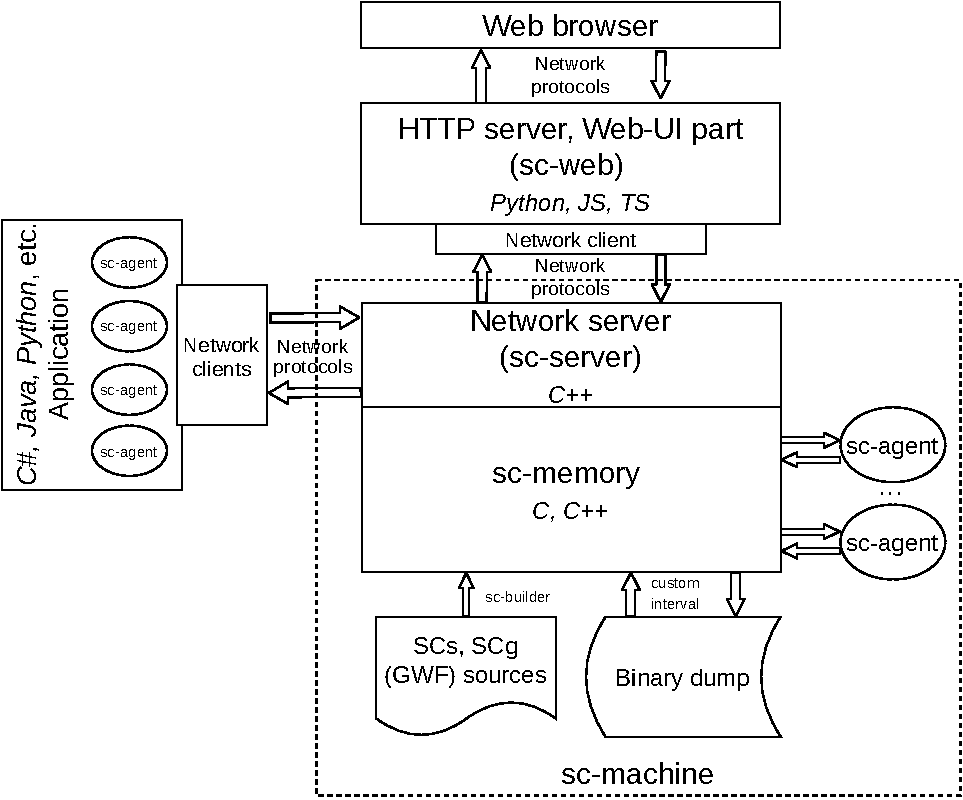
\includegraphics{figures/sd_interpreters/platform-ostis-architecture.pdf}}}
\scnaddlevel{1}
	\scnexplanation{На приведенной иллюстрации видно, что ядром платформы является \textit{Реализация sc-памяти}, с которой одновременно может взаимодействовать как с \textit{Реализацией интерпретатора sc-моделей пользовательских интерфейсов} (sc-web), так и с любыми сторонними приложениями по протоколу \textit{SCTP} или \textit{Протоколу взаимодействия с sc-памятью на основе JSON}.}
\scnaddlevel{-1}

\scnheader{Реализация sc-памяти}
\scnidtf{sc-machine}
\scntext{основной репозиторий исходных текстов}{https://github.com/ostis-dev/sc-machine.git}
\scnrelfromlist{компонент программной системы}{Реализация sc-хранилища и механизма доступа к нему;Реализация базового набора платформенно-зависимых sc-агентов и их общих компонентов;Реализация подсистемы взаимодействия с внешней средой с использованием протокола SCTP;Реализация подсистемы взаимодействия с внешней средой с использованием протоколов на основе формата JSON;Реализация вспомогательных инструментальных средств в рамках реализации sc-памяти;Реализация scp-интерпретатора}
\scntext{программная документация}{http://ostis-dev.github.io/sc-machine/}
\scnrelfromlist{используемый язык программирования}{C;C++;Python}
\scnnote{Текущий вариант \textit{Реализации sc-памяти} предполагает возможность сохранения состояния (слепка) памяти на жесткий диск и последующей загрузки из ранее сохраненного состояния. Такая возможность необходима для перезапуска системы, в случае возможных сбоев, а также при работе с исходными текстами базы знаний, когда сборка из исходных текстов сводится к формированию слепка состояния памяти, который затем помещается в \textit{Реализацию sc-памяти}.}

\scnheader{Реализация sc-хранилища и механизма доступа к нему}
\scnrelfromlist{компонент программной системы}{Реализация sc-хранилища;Реализация файловой памяти ostis-системы}
\scnrelfromlist{реализуемый механизм}{Механизм итераторов в семантической памяти;Механизм шаблонов в семантической памяти;Механизм контекстов процессов в семантической памяти;Механизм блокировок элементов семантической памяти;Механизм обработки событий в семантической памяти}

\scnheader{Реализация sc-хранилища}
\scniselement{реализация sc-хранилища на основе линейной памяти}
\scnaddlevel{1}
	\scnidtf{реализация хранилища конструкций SC-кода на основе линейной памяти}
\scnaddlevel{-1}
\scnrelfrom{иллюстрация}{\scnfileimage{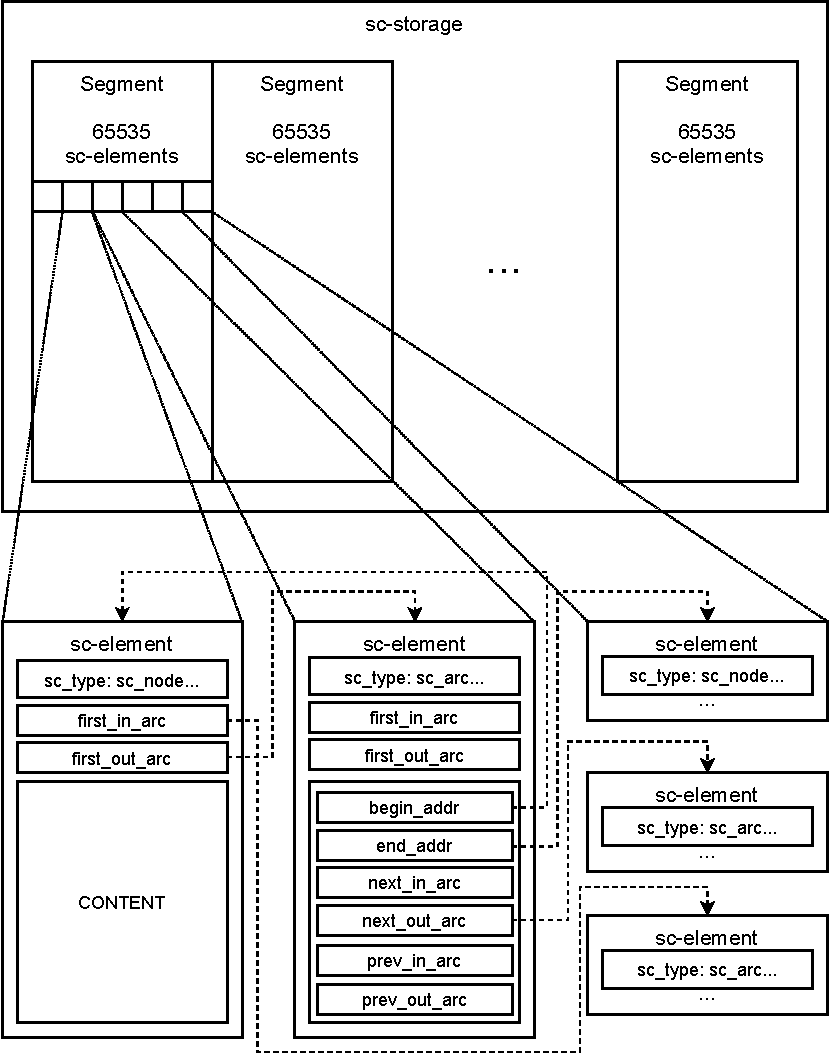
\includegraphics{figures/sd_interpreters/sc-storage.pdf}}}
\scnexplanation{В рамках данной программной реализации \textit{sc-хранилища} \scnbigspace \textit{sc-память} моделируется в виде набора \textit{сегментов}, каждый из которых состоит из фиксированного количества элементов sc-хранилища, каждый из которых соответствует конкретному sc-элементу. В настоящее время каждый сегмент состоит из $2^{16}-1=65535$ \textit{элементов sc-хранилища}.}
\scnrelfrom{класс объектов программной системы}{сегмент sc-хранилища}
\scnaddlevel{1}
	\scnnote{Максимально возможное число сегментов ограничивается настройками программной реализации sc-хранилища (в настоящее время по умолчанию установлено количество $2^{16}-1=65535$ сегментов). Таким образом, технически максимальное количество хранимых sc-элементов в текущей реализации составляет около $4.3 \times 10^{9}$ sc-элементов.}
	\scnnote{По умолчанию все сегменты физически располагаются в оперативной памяти, если объема памяти не хватает, то предусмотрен механизм выгрузки части сегментов на жесткий диск.}
	\scnrelfrom{класс объектов программной системы}{элемент sc-хранилища}
		\scnaddlevel{1}
			\scnexplanation{Каждый сегмент состоит из набора структур данных, описывающих конкретные \textit{sc-элементы} (элементов sc-хранилища). Независимо от типа описываемого sc-элемента каждый элемент sc-хранилища имеет фиксированный размер (в текущий момент -- 56 байт), что обеспечивает удобство их хранения. Таким образом, максимальный размер базы знаний в текущий момент в физическом выражении может достигнуть 223 Гб (без учета содержимого \textit{внутренних файлов ostis-системы}, хранимого на внешней файловой системе).}
		\scnaddlevel{-1}
\scnaddlevel{-1}

\scnheader{sc-адрес}
\scnidtf{адрес элемента sc-хранилища, соответствующего заданному sc-элементу, в рамках текущего состояния модели sc-памяти в составе программной реализации sc-хранилища}
\scnexplanation{Каждый элемент sc-хранилища в текущей реализации может быть однозначно задан его адресом (sc-адресом), состоящим из номера сегмента и номера sc-элемента в рамках сегмента. Таким образом, sc-адрес служит }
\scnnote{Sc-адрес никак не учитывается при обработке базы знаний на семантическом уровне и необходим только для обеспечения доступа к соответствующей структуре данных, хранящейся в линейной памяти на уровне реализации sc-хранилища.}
\scnnote{В общем случае sc-адрес элемента sc-хранилища, соответствующего заданному sc-элементу, может меняться, например, при пересборке базы знаний из исходных текстов и последующем перезапуске системы. При этом sc-адрес элемента sc-хранилища, соответствующего заданному sc-элементу, непосредственно в процессе работы системы в текущей реализации меняться не может.}
\scnnote{Для простоты будем говорить "sc-адрес sc-элемента", имея в виду \textit{sc-адрес} \scnbigspace \textit{элемента sc-хранилища}, однозначно соответствующего данному \textit{sc-элементу}.}
\scnrelfrom{обобщенная структура}{номер сегмента sc-хранилища;номер элемента sc-хранилища в рамках сегмента}

\scnheader{элемент sc-хранилища}
\scnidtf{ячейка sc-хранилища}
\scnidtf{элемент sc-хранилища, соответствующий sc-элементу}
\scnidtf{образ sc-элемента в рамках программной реализации sc-хранилища}
\scnidtf{структура данных, каждый экземпляр которой соответствует одному sc-элементу в рамках программной реализации sc-хранилища}
\scnexplanation{Каждый элемент sc-хранилища, соответствующий некоторому sc-элементу, описывается его синтаксическим типом (меткой), а также независимо от типа указывается sc-адрес первой входящей в данный sc-элемент sc-дуги и первой выходящей из данного sc-элемента sc-дуги (могут быть пустыми, если таких sc-дуг нет). 
	
Оставшиеся байты в зависимости от типа соответствующего sc-элемента (sc-узел или sc-дуга) могут использоваться либо для хранения содержимого внутреннего файла ostis-системы (может быть пустым, если sc-узел не является знаком файла), либо для хранения спецификации sc-дуги.}
\scnsubdividing{элемент sc-хранилища, соответствующий sc-узлу\\
	\scnaddlevel{1}
		\scnrelfromset{обобщенная структура}{метаинформация элемента sc-хранилища;sc-адрес первой sc-дуги, выходящей из данного sc-элемента;sc-адрес первой sc-дуги, входящей в данный sc-элемент;содержимое элемента sc-хранилища\\
		\scnaddlevel{1}
			\scnidtf{содержимое элемента sc-хранилища, соответствующего внутреннему файлу ostis-системы}
			\scnexplanation{
			Каждый sc-узел в текущей реализации может иметь содержимое (может стать \textit{внутренним файлом ostis-системы}).
			В случае, если размер содержимого внутреннего файла ostis-системы не превышает 48 байт (размер \textit{спецификации sc-дуги в рамках sc-хранилища}, например небольшой \textit{строковый идентификатор}), то это содержимое явно хранится в рамках элемента sc-хранилища в виде последовательности байт.
			В противном случае оно помещается в специальным образом организованную файловую память (за ее организацию отвечает отдельный модуль платформы, который в общем случае может быть устроен по-разному), а в рамках элемента sc-хранилища хранится уникальный адрес соответствующего файла, позволяющий быстро найти его на файловой системе.}
		\scnaddlevel{-1}}
		\scnaddlevel{1}
			\scnnote{\textit{sc-адрес первой sc-дуги, выходящей из данного sc-элемента}, \textit{sc-адрес первой sc-дуги, входящей в данный sc-элемент} и \textit{содержимое элемента sc-хранилища} в общем случае могут отсутствовать (быть нулевыми, "пустыми"), но размер элемента в байтах останется тем же.}
		\scnaddlevel{-1}
	\scnaddlevel{-1}
	;элемент sc-хранилища, соответствующий sc-дуге\\
	\scnaddlevel{1}
	\scnrelfromset{обобщенная структура}{метаинформация элемента sc-хранилища;sc-адрес первой sc-дуги, выходящей из данного sc-элемента;sc-адрес первой sc-дуги, входящей в данный sc-элемент;спецификации sc-дуги в рамках sc-хранилища\\
		\scnaddlevel{1}
			\scnrelfromset{обобщенная структура}{sc-адрес начального sc-элемента sc-дуги;sc-адрес конечного sc-элемента sc-дуги;sc-адрес следующей sc-дуги, выходящей из того же sc-элемента;sc-адрес следующей sc-дуги, входящей в тот же sc-элемент;sc-адрес предыдущей sc-дуги, выходящей из того же sc-элемента;sc-адрес предыдущей sc-дуги, входящей в тот же sc-элемент}
		\scnaddlevel{-1}}
	\scnnote{sc-ребра в текущий момент хранятся так же, как sc-дуги, то есть имеют начальный и конечный sc-элементы, отличие заключается только в \textit{метке синтаксического типа sc-элемента}. Это приводит к ряду неудобств при обработке, но sc-ребра используются в настоящее время достаточно редко.}
	\scnaddlevel{-1}}
\scnaddlevel{1}
	\scnnote{С точки зрения программной реализации структура данных для хранения sc-узла и sc-остается остается та же, но в ней меняется список полей (компонентов).\\
	Кроме того, как можно заметить каждый элемент sc-хранилища (в том числе, \textit{элемент sc-хранилища, соответствующий sc-дуге}) не хранит список sc-адресов связанных с ним sc-элементов, а хранит sc-адреса одной выходящей и одной входящей дуги, каждая из которых в свою очередь хранит sc-адреса следующей и предыдущей дуг в списке исходящих и входящих sc-дуг для соответствующих элементов.\\
	Все перечисленное позволяет:
	\begin{scnitemize}	
		\item сделать размер такой структуры фиксированным (в настоящее время 56 байт) и не зависящим от синтаксического типа хранимого sc-элемента;
		\item обеспечить возможность работы с sc-элементами без учета их синтаксического типа в случаях, когда это необходимо (например, при реализации поисковых запросов вида ``Какие sc-элементы являются элементами данного множества'', ``Какие sc-элементы непосредственно связаны с данным sc-элементом'' и т.д.);
	\end{scnitemize}}
\scnaddlevel{-1}

\scnheader{метаинформация элемента sc-хранилища}
\scnrelfromset{обобщенная структура}{метка синтаксического типа sc-элемента;метка уровня доступа sc-элемента}

\scnheader{метка синтаксического типа sc-элемента}
\scnsuperset{метка sc-узла}
\scnaddlevel{1}
	\scntext{числовое выражение в шестнадцатеричной системе}{0x1}
\scnaddlevel{-1}
\scnsuperset{метка внутреннего файла ostis-системы}
\scnaddlevel{1}
\scntext{числовое выражение в шестнадцатеричной системе}{0x2}
\scnaddlevel{-1}
\scnsuperset{метка sc-ребра общего вида}
\scnaddlevel{1}
\scntext{числовое выражение в шестнадцатеричной системе}{0x4}
\scnaddlevel{-1}
\scnsuperset{метка sc-дуги общего вида}
\scnaddlevel{1}
\scntext{числовое выражение в шестнадцатеричной системе}{0x8}
\scnaddlevel{-1}
\scnsuperset{метка sc-дуги принадлежности}
\scnaddlevel{1}
\scntext{числовое выражение в шестнадцатеричной системе}{0x10}
\scnaddlevel{-1}
\scnsuperset{метка sc-константы}
\scnaddlevel{1}
\scntext{числовое выражение в шестнадцатеричной системе}{0x20}
\scnaddlevel{-1}
\scnsuperset{метка sc-переменной}
\scnaddlevel{1}
\scntext{числовое выражение в шестнадцатеричной системе}{0x40}
\scnaddlevel{-1}
\scnsuperset{метка позитивной sc-дуги принадлежности}
\scnaddlevel{1}
\scntext{числовое выражение в шестнадцатеричной системе}{0x80}
\scnaddlevel{-1}
\scnsuperset{метка негативной sc-дуги принадлежности}
\scnaddlevel{1}
\scntext{числовое выражение в шестнадцатеричной системе}{0x100}
\scnaddlevel{-1}
\scnsuperset{метка нечеткой sc-дуги принадлежности}
\scnaddlevel{1}
\scntext{числовое выражение в шестнадцатеричной системе}{0x200}
\scnaddlevel{-1}
\scnsuperset{метка постоянной sc-дуги}
\scnaddlevel{1}
\scntext{числовое выражение в шестнадцатеричной системе}{0x400}
\scnaddlevel{-1}
\scnsuperset{метка временной sc-дуги}
\scnaddlevel{1}
\scntext{числовое выражение в шестнадцатеричной системе}{0x800}
\scnaddlevel{-1}
\scnsuperset{метка небинарной sc-связки}
\scnaddlevel{1}
\scntext{числовое выражение в шестнадцатеричной системе}{0x80}
\scnaddlevel{-1}
\scnsuperset{метка sc-структуры}
\scnaddlevel{1}
\scntext{числовое выражение в шестнадцатеричной системе}{0x100}
\scnaddlevel{-1}
\scnsuperset{метка ролевого отношения}
\scnaddlevel{1}
\scntext{числовое выражение в шестнадцатеричной системе}{0x200}
\scnaddlevel{-1}
\scnsuperset{метка неролевого отношения}
\scnaddlevel{1}
\scntext{числовое выражение в шестнадцатеричной системе}{0x400}
\scnaddlevel{-1}
\scnsuperset{метка sc-класса}
\scnaddlevel{1}
\scntext{числовое выражение в шестнадцатеричной системе}{0x800}
\scnaddlevel{-1}
\scnsuperset{метка абстрактной сущности}
\scnaddlevel{1}
\scntext{числовое выражение в шестнадцатеричной системе}{0x1000}
\scnaddlevel{-1}
\scnsuperset{метка материальной сущности}
\scnaddlevel{1}
\scntext{числовое выражение в шестнадцатеричной системе}{0x2000}
\scnaddlevel{-1}
\scnsuperset{метка константной позитивной постоянной sc-дуги принадлежности}
\scnaddlevel{1}
\scnreltoset{пересечение}{метка sc-дуги принадлежности;метка sc-константы;метка позитивной sc-дуги принадлежности;метка постоянной sc-дуги}
\scnnote{\textit{метки синтаксических типов sc-элементов} могут комбинироваться между собой для получения более частных классов меток. С точки зрения программной реализации такая комбинация выражается операцией побитового сложения значений соответствующих меток.}
\scnaddlevel{-1}
\scnsuperset{метка переменной позитивной постоянной sc-дуги принадлежности}
\scnaddlevel{1}
\scnreltoset{пересечение}{метка sc-дуги принадлежности;метка sc-переменной;метка позитивной sc-дуги принадлежности;метка постоянной sc-дуги}
\scnaddlevel{-1}
\scnnote{Числовые выражения некоторых классов меток могут совпадать. Это сделано для уменьшения размера элемента sc-хранилища за счет уменьшения максимального размера метки. Конфликт в данном случае не возникает, поскольку такие классы меток не могут комбинироваться, например \textit{метка ролевого отношения} и \textit{метка нечеткой sc-дуги принадлежности}.}
\scnnote{Важно отметить, что каждому из выделенных классов меток (кроме классов, получаемых путем комбинации других классов) однозначно соответствует порядковый номер бита в линейной памяти, что можно заметить, глядя на соответствующие числовые выражения классов меток. Это означает, что классы меток не включаются друг в друга, например, указание \textit{метки позитивной sc-дуги принадлежности} не означает автоматическое указание \textit{метки sc-дуги принадлежности}. Это позволяет сделать операции комбинирования и сравнения меток более эффективными.}

\scnheader{метка уровня доступа sc-элемента}
\scnrelfromset{обобщенная структура}{метка уровня доступа sc-элемента на чтение;метка уровня доступа sc-элемента на запись}
\scnexplanation{В текущей реализации sc-хранилища реализован механизм меток уровня доступа. Каждому элементу sc-хранилища соответствует \textit{метка уровня доступа sc-элемента на чтение} и \textit{метка уровня доступа sc-элемента на запись}, каждая из которых выражается числом от 0 до 255. 
	
В свою очередь, каждому процессу (чаще всего, соответствующему некоторому sc-агенту), который пытается получить доступ к данному элементу sc-хранилища (прочитать или изменить его) соответствует уровень доступа на чтение и запись, выраженный в том же числовом диапазоне. Указанный уровень доступа для процесса является частью \textit{контекста процесса}. Доступ на чтение или запись к элементу sc-хранилища не разрешается, если уровень доступа соответственно на чтение или запись у процесса ниже, чем у элемента sc-хранилища, к которому осуществляется доступ.

Таким образом нулевое значение \textit{метки уровня доступа sc-элемента на чтение} и \textit{метки уровня доступа sc-элемента на запись} означает, что любой процесс может получить неограниченный доступ к данному элементу sc=хранилища.}


\scnheader{Механизм итераторов в семантической памяти}
\scnheader{Механизм шаблонов в семантической памяти}
\scnheader{Механизм контекстов процессов в семантической памяти}
\scnheader{Механизм блокировок элементов семантической памяти}
\scnrelfrom{описание}{\nameref{sec:sd_agents}}
\scnheader{Механизм обработки событий в семантической памяти}

\scnheader{Реализация файловой памяти ostis-системы}
\scnauthorcomment{Пишет Денис}

\scnheader{Реализация базового набора платформенно-зависимых sc-агентов и их общих компонентов}
\scnidtf{sc-kpm}
\scnrelfromlist{компонент программной системы}{Реализация базового набора поисковых sc-агентов\\
	\scnaddlevel{1}
		\scnrelfromlist{используемый язык программирования}{C}
		\scnrelfromlist{компонент программной системы}{Реализация Абстрактного sc-агента поиска семантической окрестности заданной сущности;Реализация Абстрактного sc-агента поиска всех сущностей, частных по отношению к заданной;Реализация Абстрактного sc-агента поиска всех сущностей, общих по отношению к заданной;Реализация Абстрактного sc-агента поиска всех sc-идентификаторов, соответствующих заданной сущности;Реализация Абстрактного sc-агента поиска базовых sc-дуг, инцидентных заданному sc-элементу\\
			\scnaddlevel{1}
				\scnrelfromlist{компонент программной системы}{Реализация Абстрактного sc-агента поиска базовых sc-дуг, входящих в заданный sc-элемент;Реализация Абстрактного sc-агента поиска базовых sc-дуг, выходящих из заданного sc-элемента;Реализация Абстрактного sc-агента поиска базовых sc-дуг, входящих в заданный sc-элемент, с указанием множеств, которым принадлежат эти sc-дуги;Реализация Абстрактного sc-агента поиска базовых sc-дуг, выходящих из заданного sc-элемента, с указанием множеств, которым принадлежат эти sc-дуги}
			\scnaddlevel{-1}}
	\scnaddlevel{-1}
	;Реализация базового механизма сборки информационного мусора\\
	\scnaddlevel{1}
		\scnrelfromlist{используемый язык программирования}{C}	
		\scnnote{Текущая реализация механизма сборки информационного мусора, содержит один sc-агент, реагирующий на явное добавление какого-либо sc-элемента во множество ``информационный мусор'' и осуществляющий физическое удаление этого sc-элемента из sc-памяти}
	\scnaddlevel{-1}
	;Реализация базового набора интерфейсных sc-агентов\\
	\scnaddlevel{1}
	\scnrelfromlist{используемый язык программирования}{C++}	
	\scnrelfromlist{компонент программной системы}{Реализация Абстрактного sc-агента обработки команд пользовательского интерфейса;Реализация Абстрактного sc-агента трансляции из внутреннего представления знаний во промежуточный транспортный формат\\
	\scnaddlevel{1}
		\scnnote{В настоящее время используется подход, при котором независимо от формы внешнего представления информации, информация хранимая в sc-памяти вначале транслируется в промежуточный транспортный формат на базе JSON, который затем обрабатывается sc-агентами пользовательского интерфейса, входящими в состав \textit{Реализации интерпретатора sc-моделей пользовательских интерфейсов}}
	\scnaddlevel{1}
	}
	\scnaddlevel{-1}
}

\scnheader{SCTP}
\scnidtf{Semantic Code Transfer Protocol}
\scnrelboth{аналогия}{HTTP}
\scnexplanation{SCTP представляет собой \textit{бинарный протокол}, позволяющий осуществлять операции чтения (поиска) и редактирования конструкций, хранящихся в sc-памяти, а также отслеживать события, происходящие в sc-памяти.

Взаимодействие между клиентом и сервером на протоколе SCTP осуществляется путем обмена \textit{sctp-командами}, каждая из которых представляет собой набор байт, предназначенный для машинной обработки (но не восприятия человеком).
}

\scnheader{sctp-команда}
\scnrelfromset{обобщенная декомпозиция}{заголовок sctp-команды\\
	\scnaddlevel{1}
		\scnidtf{часть sctp-команды, в которой указан её тип и некоторая дополнительная информация о ней}
	\scnaddlevel{-1}
	;аргументы sctp-команды\\
	\scnaddlevel{1}
		\scnidtf{часть sctp-команды, которая содержит её аргументы и размер которой может быть разным в зависимости от типа команды.}
	\scnaddlevel{-1}}
\scnrelfromlist{включение;пример}{sctp-команда удаления sc-элемента с указанным sc-адресом;sctp-команда создания нового sc-узла указанного типа;sctp-команда получения начального и конечного элемента sc-дуги}
\scnnote{Выполнение каждой sctp-команды предполагает наличие sctp-результата, однозначно соответствующего данной команде.}

\scnheader{SCTP}
\scntext{программная документация}{http://ostis-dev.github.io/sc-machine/net/sctp/}
\scnrelfromlist{недостаток}{\scnfileitem{Команды протокола SCTP являются низкоуровневыми (ориентированы на работу с единичными sc-элементами или простейшими sc-конструкциями из 3 или 5 элементов). Это приводит к тому, что выполнение даже несложного преобразования в базе знаний или ассоциативный поиск по набору взаимосвязанных конструкций выражаются в виде достаточно большого набора sctp-команд. С учетом того, что для каждой команды существует sctp-результат, также пересылаемый по сети, это излишне нагружает сеть и сильно ухудшает производительность системы в целом. Кроме того, производительность системы начинает сильно зависеть от пропускной способности сети.};
\scnfileitem{Протокол SCTP не предназначен для восприятия человеком}}
\scnrelfromlist{достоинство}{\scnfileitem{Протокол SCTP является кросс-платформенным};\scnfileitem{Протокол SCTP может быть достаточно просто реализован практически на любом языке программирования}}
\scnrelfromlist{обобщенная реализация}{sctp-сервер\\
	\scnaddlevel{1}
		\scnexplanation{Sctp-сервер обрабатывает sctp-команды, приходящие от разных sctp-клиентов, и обеспечивает их интерпретацию в sc-памяти.}
	\scnaddlevel{-1}
	;sctp-клиент\\
	\scnaddlevel{1}
		\scnexplanation{Sctp-клиенты в общем случае могут быть реализованы на разных языках программирования и иметь разный программный интерфейс. По сути задачей sctp-клиента является преобразование высокоуровневых команд представленных в форме, удобной программисту, в одну или более низкоуровневых sctp-команд, отправка их на сервер, ожидание sctp-результата и его интерпретация.}
	\scnaddlevel{-1}}

\scnheader{Реализация подсистемы взаимодействия с внешней средой с использованием протокола SCTP}
\scnrelfromlist{компонент программной системы}{Реализация sctp-сервера;Реализация sctp-клиента\\
	\scnaddlevel{1}
	\scnnote{\textit{Реализация подсистемы взаимодействия с внешней средой с использованием протокола SCTP} включает в себя \textit{Реализацию sctp-клиента} на языке C++, в то же время есть другие реализации \textit{sctp-клиентов} в рамках того же программного варианта реализации платформы, например, в рамках \textit{Реализации интерпретатора sc-моделей пользовательских интерфейсов}.}
	\scnaddlevel{-1}}

\scnheader{Реализация подсистемы взаимодействия с внешней средой с использованием протоколов на основе формата JSON}
\scnexplanation{В связи с большим числом недостатков протокола SCTP было принято решение о разработке другого протокола на основе какого-либо общепринятого текстового транспортного формата. В качестве такого формата был выбран формат JSON.}
\scnrelto{реализация}{Протокол взаимодействия с sc-памятью на основе JSON}
\scnaddlevel{1}
\scnnote{Данный протокол пока не имеет собственного названия}
\scntext{программная документация}{http://ostis-dev.github.io/sc-machine/http/websocket/}
\scnexplanation{В рамках \textit{Протокола взаимодействия с sc-памятью на основе JSON} каждая команда представляет собой json-объект, в котором указываются идентификатор команда, тип команды и ее аргументы. В свою очередь ответ на команду также представляет собой json-объект, в котором указываются идентификатор команды, ее статус (выполнена успешно/безуспешно) и результаты. Структура аргументов и результатов команды определяется типом команды.}
\scnrelfromlist{достоинство}{\scnfileitem{JSON является общепринятым открытым форматом, для работы с которым существует большое количество библиотек для популярных языков программирования. Это, в свою очередь, упрощает реализацию клиента и сервера для протокола, построенного на базе JSON.};
\scnfileitem{Реализация протокола на базе JSON не накладывает принципиальных ограничений на объем (длину) каждой команды, в отличие от бинарного протокола. Таким образом, появляется возможность использования неатомарных команд, позволяющих, например, за один акт пересылки такой команды по сети создать сразу несколько sc-элементов. Важными примерами таких команд являются  \textit{Команда генерации по произвольному образцу} и \textit{Команда поиска по произвольному образцу}.}}
\scnaddlevel{-1}

\scnheader{Реализация вспомогательных инструментальных средств в рамках реализации sc-памяти}
\scnrelfrom{компонент программной системы}{Реализация сборщика базы знаний из исходных текстов, записанных в SCs-коде}
\scnaddlevel{1}
\scnidtf{sc-builder}
\scnrelfrom{используемый язык}{SCs-код}
\scnexplanation{Сборщик базы знаний из исходных текстов позволяет осуществить сборку базы знаний из набора исходных текстов, записанных в SCs-коде с ограничениями (см. \textit{Раздел **про исходные тексты**}) в бинарный формат, воспринимаемый \textit{Реализацией sc-памяти}. При этом возможна как сборка "с нуля"{} (с уничтожением ранее созданного слепка памяти), так и аддитивная сборка, когда информация, содержащаяся в заданном множестве файлов, добавляется к уже имеющемуся слепку состояния памяти.

В текущей реализации сборщик осуществляет "склеивание"{} ("слияние"{}) sc-элементов, имеющих на уровне исходных текстов одинаковые \textit{системные sc-идентификаторы}.}
\scnaddlevel{-1}

\scnheader{Реализация интерпретатора sc-моделей пользовательских интерфейсов}
\scnidtf{sc-web}
\scnrelfromlist{используемый язык программирования}{JavaScript;TypeScript;Python}
\scnrelfrom{иллюстрация}{\scnfileimage{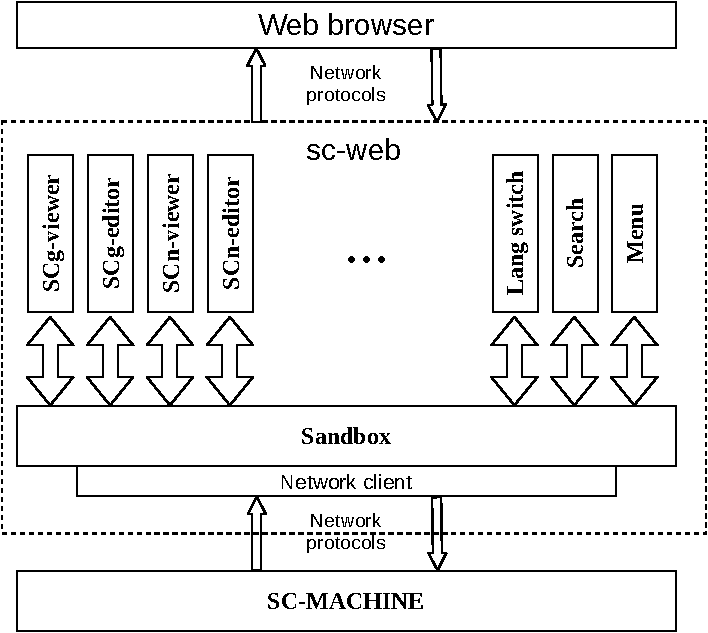
\includegraphics{figures/sd_interpreters/sc-web-new-arch.pdf}}}
\scnaddlevel{1}
	\scnexplanation{На данной иллюстрации показан планируемый вариант архитектуры \textit{Реализация интерпретатора sc-моделей пользовательских интерфейсов}, важным принципом которой является простота и однотипность подключения любых компонентов пользовательского интерфейса (редакторов, визуализаторов, переключателей, команд меню и т.д.). Для этого реализуется программная прослойка Sandbox, в рамках которой реализуются низкоуровневые операции взаимодействия с серверной частью и которая обеспечивает более удобный программный интерфейс для разработчиков компонентов.}
\scnaddlevel{-1}
\scnrelfromset{недостатки текущей реализации}{\scnfileitem{Отсутствие единого унифицированного механизма клиент-серверного взаимодействия. Часть компонентов (визуализатор sc-текстов в SCn-коде, команды меню и др.) работают по протоколу HTTP, часть по протоколу SCTP, это приводит к значительным трудностям при развитии платформы. 
Протокол HTTP предполагает четкое разделение активного клиента и пассивного сервера, который отвечает на запросы клиентов. Таким образом, сервер (в данном случае -- sc-память) практически не имеет возможности по своей инициативе отправить сообщение клиенту, что повышает безопасность системы, но значительно снижает ее интерактивность. Кроме того, такой вариант реализации затрудняет реализацию принятого в Технологии OSTIS многоагентного подхода, в частности, затрудняет реализацию sc-агентов на стороне клиента. Указанные проблемы могут быть решены путем постоянного мониторинга определенных событий со стороны клиента, однако такой вариант неэффективен.
Кроме того, часть интерфейса работает напрямую с sc-памятью (по протоколу SCTP), а часть -- через прослойку на базе библиотеки tornado для языка программирования Python, что приводит к дополнительным зависимостям от сторонних библиотек.};
\scnfileitem{Часть компонентов (например, поле поиска по идентификатору) реализована сторонними средствами и практически никак не связана с sc-памятью. Это затрудняет развитие платформы.};
\scnfileitem{Текущая \textit{Реализация интерпретатора sc-моделей пользовательских интерфейсов} ориентирована только на ведение диалога с пользователем (в стиле вопрос пользователя -- ответ системы). Не поддерживаются такие очевидно необходимые ситуации, как выполнение команды, не предполагающей ответа\char59~возникновение ошибки или отсутствие ответа\char59~необходимость задания вопроса системой пользователю и т.д.};
\scnfileitem{Ограничена возможность взаимодействия пользователя с системой без использования специальных элементов управления. Например, можно задать вопрос системе, нарисовав его в SCg-коде, но ответ пользователь не увидит, хотя в памяти он будет сформирован соответствующим агентом.;
Большая часть технологий, использованных при реализации платформы, к настоящему моменту устарела, что затрудняет развитие платформы.};
\scnfileitem{Идея платформенной независимости пользовательского интерфейса (построения sc-модели пользовательского интерфейса) реализована не в полной мере. Полностью описать sc-модель пользовательского интерфейса (включая точное размещение, размеры, дизайн компонентов, их поведение и др.) в настоящее время скорее всего окажется затруднительно из-за ограничений производительности, однако вполне возможно реализовать возможность задания вопросов ко всем компонентам интерфейса, изменить их расположение и т.д., однако эти возможности нельзя реализовать в текущей версии реализации платформы.};
\scnfileitem{Интерфейсная часть работает медленно из-за недостатков  протокола SCTP и некоторых недостатков реализации серверной части на языке Python.;
Не реализован механизм наследования при добавлении новых внешних языков. Например, добавление нового языка даже очень близкого к SCg-коду требует физического копирования кода компонента и внесение соответствующих изменений, при этом получаются два никак не связанных между собой компонента, которые начинают развиваться независимо друг от друга.};
\scnfileitem{Слабый уровень задокументированности текущей \textit{Реализации интерпретатора sc-моделей пользовательских интерфейсов}.}}
\scnrelfromset{требования к будущей реализации}{\scnfileitem{Унифицировать принципы взаимодействия всех компонентов интерфейса с \textit{Реализацией sc-памяти}, независимо от того, к какому типу относится компонент. Например, список команд меню должен формироваться через тот же механизм, что и ответ на запрос пользователя, и команда редактирования, сформированная пользователем, и команда добавления нового фрагмента в базу знаний и т.д.};
\scnfileitem{Унифицировать принципы взаимодействия пользователей с системой независимо от способа взаимодействия и внешнего языка. Например, должна быть возможность задания вопросов и выполнения других команд прямо через SCg/SCn интерфейс. При этом необходимо учитывать принципы редактирования базы знаний, чтобы пользователя не мог под видом задания вопроса внести новую информацию в согласованную часть базы знаний.};
\scnfileitem{Унифицировать принципы обработки событий, происходящих при взаимодействии пользователя с компонентами интерфейса -- поведение кнопок и других интерактивных компонентов должно задаваться не статически сторонними средствами, а реализовываться в виде агента, который, тем не менее, может быть реализован произвольным образом (не обязательно на платформенно-независимом уровне). Любое действие, совершаемое пользователем, на логическом уровне должно трактоваться и обрабатываться как инициирование агента.};
\scnfileitem{Обеспечить возможность выполнять команды (в частности, задавать вопросы) с произвольным количеством аргументов, в том числе -- без аргументов.};
\scnfileitem{Обеспечить возможность отображения ответа на вопрос по частям, если ответ очень большой и для отображения требуется много времени.};
\scnfileitem{Каждый отображаемый компонент интерфейса должен трактоваться как изображение некоторого sc-узла, описанного в базе знаний. Таким образом, пользователь должен иметь возможность задания произвольных вопросов к любым компонентам интерфейса.};
\scnfileitem{Максимально упростить и задокументировать механизм добавления новых компонентов.};
\scnfileitem{Обеспечить возможность добавления новых компонентов на основе имеющихся без создания независимых копий. Например, должна быть возможность создать компонент для языка, расширяющего язык SCg новыми примитивами, переопределять принципы размещения sc-текстов и т.д.};
\scnfileitem{Свести к минимуму зависимость от сторонних библиотек.};
\scnfileitem{Свести к минимуму использование протокола HTTP (начальная загрузка общей структуры интерфейса), обеспечить возможность равноправного двустороннего взаимодействия серверной и клиентской части.};
\scnfileitem{Полностью отказаться от протокола SCTP, перейти на протокол на базе JSON, задокументировать его.}}
\scnaddlevel{1}
	\scnnote{Очевидно, что реализация большинства из приведенных требований связана не только с собственно вариантом реализации платформы, но и требует развития теории логико-семантических моделей пользовательских интерфейсов и уточнения в рамках нее общих принципов организации пользовательских интерфейсов ostis-систем. Однако, принципиальная возможность реализации таких моделей должна быть учтена в рамках реализации платформы.}
\scnaddlevel{-1}

\scnheader{Реализация scp-интерпретатора}
\scnrelfromlist{используемый язык программирования}{C++}
\scnrelfromlist{компонент программной системы}{Реализация Абстрактного sc-агента создания scp-процессов;Реализация Абстрактного sc-агента интерпретации scp-операторов\\
	\scnaddlevel{1}
	\scnrelfromlist{компонент программной системы}{Реализация Абстрактного sc-агента интерпретации scp-операторов генерации конструкций;Реализация Абстрактного sc-агента интерпретации scp-операторов ассоциативного поиска конструкций;Реализация Абстрактного sc-агента интерпретации scp-операторов удаления конструкций;Реализация Абстрактного sc-агента интерпретации scp-операторов проверки условий		;Реализация Абстрактного sc-агента интерпретации scp-операторов управления значениями операндов;Реализация Абстрактного sc-агента интерпретации scp-операторов управления scp-процессами;Реализация Абстрактного sc-агента интерпретации scp-операторов управления событиями;Реализация Абстрактного sc-агента интерпретации scp-операторов обработки содержимых числовых файлов;Реализация Абстрактного sc-агента интерпретации scp-операторов обработки содержимых строковых файлов}
	\scnaddlevel{-1}
	;Реализация Абстрактного sc-агента синхронизации процесса интерпретации scp-программ;Реализация Абстрактного sc-агента уничтожения scp-процессов;Реализация Абстрактного sc-агента синхронизации событий в sc-памяти и ее реализации}
\scnnote{Текущая \textit{Реализация scp-интерпретатора} не включает в себя специализированных средств для работы с блокировками, поскольку механизм блокировок элементов sc-памяти реализован на более низком уровне в рамках \textit{Реализация sc-хранилища и механизма доступа к нему}}

\scnendstruct

\end{SCn}

\scsubsubsection{Предметная область и онтология семантических ассоциативных компьютеров для ostis-систем}
\begin{SCn}

\scnsectionheader{Предметная область и онтология семантических ассоциативных компьютеров для ostis-систем}

\scnstartsubstruct

\scnheader{Предметная область и онтология семантических ассоциативных компьютеров для ostis-систем}
\scnsdmainclasssingle{***}
\scnsdclass{***}
\scnsdrelation{***}

\scnheader{семантический ассоциативный компьютер}
\scnidtf{аппаратно реализованный интерпретатор семантических моделей (sc-моделей) компьютерных систем}
\scnidtf{семантический ассоциативный компьютер, управляемый знаниями}
\scnidtf{компьютер с нелинейной структурно перестраиваемой (графодинамической) ассоциативной памятью, переработка информации в которой сводится не к изменению состояния элементов памяти, а к изменению конфигурации связей между ними}
\scnidtf{sc-компьютер}
\scnidtf{scp-компьютер}
\scnidtf{компьютер, управляемый знаниями, представленными в SC-коде}
\scnidtf{компьютер, ориентированный на обработку текстов SC-кода}

\filemodetrue
\scnrelfromlist{принцип}{
нелинейная память — каждый элементарный фрагмент хранимого в памяти текста может быть инцидентен неограниченному числу других элементарных фрагментов этого текста;
структурно перестраиваемая (реконфигурируемая) память — процесс отработки хранимой в памяти информации сводится не только к изменению состояния элементов, но и к реконфигурации связей между ними;
в качестве внутреннего способа кодирования знаний, хранимых в памяти семантического ассоциативного компьютера, используется универсальный (!) способ нелинейного (графоподобного) смыслового представления знаний, названный нами SC-кодом (семантическим, смысловым компьютерным кодом);
обработка информации осуществляется коллективом агентов, работающих над общей памятью. Каждый из них реагирует на соответствующую ему ситуацию или событие в памяти (компьютер, управляемый хранимыми знаниями);
есть программно реализуемые агенты, поведение которых описывается хранимыми в памяти агентно-ориентированными программами, которые интерпретируются соответствующими коллективами агентов;
есть базовые агенты, которые не могут быть реализованы программно (в частности, это агенты интерпретации агентных программ, базовые рецепторные агенты-датчики, базовые эффекторные агенты);
все агенты работают над общей памятью одновременно. Более того, если для какого-либо агента в некоторый момент времени в различных частях памяти возникает сразу несколько условий его применения, разные акты указанного агента в разных частях памяти могут выполняться одновременно (акт агента — это неделимый, целостный процесс деятельности агента);
для того, чтобы акты агентов, параллельно выполняемые в общей памяти не "мешали"\ друг другу, для каждого акта в памяти фиксируется и постоянно актуализируется его текущее состояние. То есть каждый акт сообщает всем остальным о своих намерениях и пожеланиях, которым остальные агенты не должны препятствовать (например, это различного рода блокировки используемых элементов семантической памяти);
кроме того, агенты (точнее, выполняемые ими акты) должны соблюдать "этику"\,, стараясь не в ущерб себе создавать максимально благоприятные условия для других агентов (актов), например, не жадничать, быстрее возвращать, не захватывать (не блокировать) лишние элементы памяти, как можно скорее освобождать (деблокировать) заблокированные элементы памяти;
процессор и память семантического ассоциативного компьютера глубоко интегрированы и составляют единую процессоро-память. Процессор семантического ассоциативного компьютера равномерно "распределен"\ по его памяти так, что процессорные элементы одновременно являются и элементами памяти компьютера. Обработка информации в семантическом ассоциативном компьютере сводится к реконфигурации каналов связи между процессорными элементами,  следовательно память такого компьютера есть не что иное, как \uline{коммутатор} (!) указанных каналов связи. Таким образом, текущее состояние конфигурации этих каналов связи и есть текущее состояние обрабатываемой информации}
\filemodefalse

\scnendstruct

\end{SCn}

\scsubsection{Предметная область и онтология многократно используемых компонентов ostis-систем}
\begin{SCn}

\scnsectionheader{\currentname}
\scnrelfromlist{подраздел}{Предметная область и онтология многократно используемых компонентов баз знаний ostis-систем;Предметная область и онтология многократно используемых внутренних агентов ostis-систем;Предметная область и онтология многократно используемых интерпретируемых ostis-системами методов;Предметная область и онтология многократно используемых компонентов интерфейсов ostis-систем;Библиотека многократно используемых встраиваемых ostis-систем}

\scnstartsubstruct

\scnheader{Предметная область многократно используемых компонентов ostis-систем}
\scnsdmainclasssingle{...}
\scnsdclass{}
\scnsdrelation{}

\scnheader{Библиотека многократно используемых компонентов OSTIS}
\scnidtf{Библиотека OSTIS}
\scnidtf{многократно используемый компонент OSTIS}
\scnidtf{многократно используемый компонент интеллектуальных систем, построенных по Технологии OSTIS}
\scnexplanation{Под \textbf{\textit{многократно используемым компонентом OSTIS}} понимается компонент некоторой ostis-системы, который может быть использован в рамках другой ostis-системы. Для этого необходимо выполнение как минимум двух условий:
\begin{scnitemize}
    \item есть техническая возможность встроить компонент в другую ostis-систему, либо путем физического копирования, переноса и встраивания его в проектируемую систему, либо использования компонента, размещенного в исходной системе наподобие сервиса, то есть без явного копирования и переноса компонента. Трудоемкость встраивания зависит, в том числе, от реализации компонента;
    \item использование компонента в каких-либо ostis-системах, кроме материнской, является целесообразным, то есть компонентом не может быть частное решение, ориентированное на узкий круг задач. Стоит, однако, отметить, что в общем случае практически каждое решение может быть использовано в каких-либо других системах, круг которых определяется степенью общности и предметной зависимостью такого решения.
\end{scnitemize}
С формальной точки зрения каждый \textbf{\textit{многократно используемый компонент OSTIS}} представляет собой \textit{структуру}, которая содержит все те (и только те) \textit{sc-элементы}, которые необходимы для функционирования компонента в \textit{дочерней ostis-системе} и, соответственно, должны быть в нее скопированы при включении компонента в одну из таких систем. Конкретный состав данной \textit{структуры} зависит от типа компонента и уточняется для каждого типа отдельно. По сути, данная \textit{структура} представляет собой эталон или образец, который копируется при включении соответствующего компонента в дочернюю систему.

Каждый \textbf{\textit{многократно используемый компонент OSTIS}} может быть атомарным, либо неатомарным, то есть состоять из более простых самодостаточных компонентов.

В зависимости от типа компонента в его составе, т.е. в составе соответствующей \textit{структуры}, могут дополнительно вводиться роли некоторых \textit{sc-элементов}, если это необходимо. Например, в случае \textit{многократно используемого sc-агента}, сам \textit{sc-узел}, обозначающий \textit{sc-агент}, будет являться \textit{ключевым sc-элементом'} в рамках компонента.

В каждый момент времени в текущем состоянии \textit{sc-памяти} каждый многократно используемый компонент может представлен полностью, т.е. в памяти явно присутствуют все \textit{sc-дуги принадлежности}, соединяющие соответствующую компоненту \textit{структуру} и все ее элементы, или представлен неявно, например, при помощи указания \textit{ключевых sc-элементов'} данного компонента или путем задания декомпозиции данного компонента на более частные.

Каждый \textbf{\textit{многократно используемый компонент OSTIS}} имеет формальную спецификацию, то есть некоторую \textit{семантическую окрестность}, характеризующую данный компонент. На основе формальной спецификации осуществляется поиск подходящего компонента в библиотеке, сравнение его с другими компонентами и т.д.

Данная спецификация включает, как минимум:
\begin{scnitemize}
    \item Информацию об авторстве компонента, то есть связь компонента со знаком автора (физического лица, коллектива и т.д.) при помощи отношения \textit{автор*};
    \item Информацию о типе компонента, посредством указания принадлежности компонента какому-либо классу многократно используемых компонентов;
    \item Описание назначения компонента, его особенностей;
    \item Историю изменений компонента по версиям;
    \item При необходимости сведения об открытости компонента и возможностях его использования в различных системах с точки зрения проприетарности;
    \item И др.
\end{scnitemize}
Не следует путать понятия \textbf{версии компонента} и \textbf{модификации компонента}. Версии отражают историю изменений компонента (как правило, какие-либо улучшения или устранения ошибок). Модификации представляют собой функционально эквивалентные, но разные варианты реализации одного и того же компонента, которые могут быть синтаксически эквивалентны (то есть быть реализованными при помощи одних и тех же языковых средств). В качестве примера синтаксически не эквивалентной модификации можно привести реализацию одного и того же \textit{sc-агента} на одном и том же языке но с отличиями в алгоритме, в качестве синтаксически эквивалентной модификации – платформенно-зависимую и платформенно-независимую реализацию одного и того же \textit{sc-агента}.

В общем случае система \textit{IMS} как материнская система взаимодействует со всеми своими \textit{дочерними ostis-системами} (с системами, построенными по \textit{Технологии OSTIS}), обеспечивая в дочерних системах автоматическое обновление версий \textit{многократно используемых компонентов OSTIS}. Любая дочерняя система, построенная по \textit{Технологии OSTIS}, в том числе, выполняет роль посредника между разработчиком такой системы и системой \textit{IMS}. Разработчик имеет возможность выбрать интересующий его компонент или набор компонентов в одной из библиотек, и включить их в разрабатываемую дочернюю систему. Таким образом, можно говорить о том, что \textbf{разработчик} систем, построенных по \textit{Технологии OSTIS}, является \textbf{конечным пользователем} системы \textit{IMS}. При обеспечении такого механизма взаимодействия между системами, построенными на основе \textit{Технологии OSTIS}, указанные системы формируют Глобальную базу знаний, в пределах которой различные системы могут координироваться и решать более глобальные задачи, нежели это может делать одна отдельно взятая система. В случае намеренной изоляции какой-либо из систем из такого коллектива, в частности, потери связи с системой \textit{IMS}, она теряет возможность получать своевременные обновления используемых компонентов, а также использовать знания, накопленные в других системах для решения стоящих перед ней задач. Речь в данном случае идет не только о физической изоляции рассматриваемой системы, которая может быть легко устранена, а о рассогласовании знаний данной системы и других систем, что не позволит безболезненно интегрировать компоненты из библиотек в такую систему. Таким образом, разработчик каждой системы обязан следить за тем, чтобы его система находилась в постоянном согласовании с глобальным смысловым пространством, что позволит пользователям в полной мере использовать все возможности коллектива систем.

В некоторых случаях может оказаться, что для использования одного \textbf{\textit{многократно используемого компонента OSTIS}} целесообразно или даже необходимо дополнительно использовать несколько других \textbf{\textit{многократно используемых компонентов OSTIS}}. Например, может оказаться целесообразным вместе с каким либо \textit{sc-агентом информационного поиска} использовать соответствующую команду интерфейса, которая представлена отдельным компонентом и позволит пользователю задавать вопрос для указанного \textit{sc-агента} через интерфейс системы. В таких случаях для связи компонентов используется отношение \textit{сопутствующий компонент*}. Наличие таких связей позволяет устранить возможные проблемы неполноты знаний и навыков в дочерней системе, из-за которых какие-либо из компонентов могут не выполнять свои функции. Связки отношения \textit{сопутствующий компонент*} связывают \textbf{\textit{многократно используемые компоненты OSTIS}}, которые целесообразно или необходимо использовать в дочерней системе вместе. При этом каждая связка направляется от зависящего компонента к зависимому. Каждая такая связка может дополнительно быть снабжена \textit{комментарием} или \textit{пояснением}, отражающим суть указываемой зависимости.

Включение компонента в \textit{дочернюю ostis-систему} в самом общем случае состоит из следующих этапов:
\begin{scnitemize}
    \item поиск подходящего компонента (или набора компонентов) во множестве библиотек, входящих в состав \textit{IMS}. Для облегчения задачи поиска могут быть реализованы специализированные поисковые агенты. В любом случае, поиск и выделение компонента будет осуществляться на основе спецификации компонента. Данный этап с точки зрения пользователя не зависит от типа компонента и особенностей его реализации. Конкретные действия на следующих  этапах сильно зависят от реализации и типа компонента и будут более детально описаны при рассмотрении подклассов \textbf{\textit{многократно используемых компонентов OSTIS}};
    \item выделение компонента (или набора компонентов) в рамках \textit{IMS} в виде, удобном для транспортировки в \textit{дочернюю ostis-систему} (при необходимости – создание физической копии компонента);
    \item транспортировка выделенного компонента в \textit{дочернюю sc-систему};
    \item интеграция компонента в \textit{дочернюю ostis-систему}. Если в системе уже использовалась более старая версия компонента, то необходимо произвести либо локальное обновление, либо полную замену устаревшей версии компонента. Дальнейший процесс интеграции зависит от типа компонента, например, в случае добавления нового \textit{sc-агента} он должен быть помечен как \textit{активный sc-агент} и т.п.
\end{scnitemize}

Для обеспечения возможности встраивания \textbf{\textit{многократно используемых компонентов OSTIS}} в дочернюю систему, каждая такая система обязана иметь в своем составе средства, обеспечивающие интеграцию новых компонентов в систему и, при необходимости, удаление устаревших версий этих компонентов (или автоматического локального обновления компонентов до более новой версии).}

\scnauthorcomment{разбиение согласовать со структурой разделов или убрать вообще}

\scnreltoset{разбиение}{Семейство платформ интерпретации sc-моделей компьютерных систем
;Библиотека многократно используемых компонентов sc-моделей баз знаний;Библиотека шаблонов типовых компонентов sc-моделей компьютерных систем;Библиотека многократно используемых компонентов абстрактных sc-машин;Библиотека многократно используемых компонентов sc-моделей интерфейсов компьютерных систем;Библиотека типовых подсистем компьютерных систем, разрабатываемых по Технологии OSTIS}
\scnreltoset{разбиение}{атомарный многократно используемый компонент OSTIS;неатомарный многократно используемый компонент OSTIS}
\scnreltoset{разбиение}{платформенно-зависимый многократно используемый компонент OSTIS;платформенно-независимый многократно используемый компонент OSTIS}

\scnheader{шаблон типового компонента OSTIS}

\scnheader{атомарный многократно используемый компонент OSTIS}
\scnexplanation{Под \textbf{\textit{атомарным многократно используемым компонентом OSTIS}} подразумевается компонент, который в текущем состоянии библиотеки компонентов рассматривается как неделимый, то есть не содержит в своем составе других компонентов, представленных в какой-либо из библиотек компонентов в рамках \textit{IMS}. В общем случае атомарный компонент может перейти в разряд неатомарных в случае, если будет принято решение выделить какую-то из его частей в качестве отдельного компонента. Все вышесказанное, однако, не означает, что даже в случае его платформенной независимости, атомарный компонент всегда хранится в sc-памяти как сформированная sc-структура. Например, \textit{платформенно-независимая реализация sc-агента} всегда будет представлена набором \textit{scp-программ}, но будет \textbf{\textit{атомарным многократно используемым компонентом OSTIS}} в случае, если ни одна из этих программ не будет представлять интереса как самостоятельный компонент.}

\scnheader{неатомарный многократно используемый компонент OSTIS}
\scnexplanation{Под \textbf{\textit{неатомарным многократно используемым компонентом OSTIS}} подразумевается компонент, который в текущем состоянии библиотеки компонентов содержит в своем составе более простые компоненты, представленные в каких-либо библиотеках компонентов в рамках \textit{IMS}. В общем случае неатомарный компонент может перейти в разряд атомарных в случае, если будет принято решение по каким-либо причинам исключить все его части из рассмотрения в качестве отдельных компонентов.

Следует отметить, что неатомарный компонент необязательно должен складываться полностью из других компонентов, в его состав могут также входить и части, не являющиеся самостоятельными компонентами. Например, в состав реализованного на \textit{языке SCP sc-агента}, являющего \textbf{\textit{неатомарным многократно используемым компонентом}} могут входить как \textit{scp-программы}, которые могут являться \textit{многократно используемыми компонентами} (а могут и не являться), а также \textit{агентная scp-программа}, которая не имеет смысла как многократно используемый компонент.}

\scnheader{платформенно-зависимый многократно используемый компонент OSTIS}
\scnexplanation{Под \textbf{\textit{платформенно-зависимым многократно используемым компонентом OSTIS}} понимается компонент, частично или полностью реализованный при помощи каких-либо сторонних с точки зрения \textit{Технологии OSTIS} средств. Основной недостаток платформенно-зависимых компонентов состоит в том, что их интеграция в интеллектуальные системы может сопровождаться дополнительными трудностями, зависящими от конкретных средств реализации компонента. В качестве возможного преимущества \textbf{\textit{платформенно-зависимых многократно используемых компонентов OSTIS}} можно выделить их, как правило, более высокую производительность за счет реализации их на более приближенном к платформе уровне.

В общем случае \textbf{\textit{платформенно-зависимый многократно используемый компонент OSTIS}}  может поставляться как в виде набора исходных кодов, так и бинарном виде, например в виде скомпилированной библиотеки.

Процесс интеграции \textbf{\textit{платформенно-зависимого многократно используемого компонента OSTIS}} в дочернюю систему, разработанную по \textit{Технологии OSTIS}, сильно зависит от технологий реализации данного компонента и в каждом конкретном случае может состоять из различных этапов.

Для того чтобы \textbf{\textit{платформенно-зависимый многократно используемый компонент OSTIS}} мог быть успешно встроен в дочернюю систему, необходимо выполнение следующих условий:
\begin{scnitemize}
    \item в состав \textit{структуры}, соответствующей компоненту, должны входить знаки \textit{файлов}, обозначающих исходные тексты компонента или уже собранной его версии, то есть ссылки на внешние ресурсы или явно включенные в систему файлы компонента в виде указанных \textit{файлов};
    \item каждый \textbf{\textit{платформенно-зависимый многократно используемый компонент OSTIS}} должен иметь соответствующую подробную, корректную и понятную инструкцию по его установке и внедрению в дочернюю систему;
\end{scnitemize}
}

\scnheader{платформенно-независимый многократно используемый компонент OSTIS}
\scnexplanation{Под \textbf{\textit{платформенно-независимым многократно используемым компонентом OSTIS}} понимается компонент, который целиком и полностью представлен в \textit{SC-коде}. В случае \textit{неатомарного многократно используемого компонента} это означает, что все более простые компоненты, входящие в его состав также обязаны быть \textbf{\textit{платформенно-независимыми многократно используемыми компонентами OSTIS}}.

Процесс интеграции \textbf{\textit{платформенно-зависимого многократно используемого компонента OSTIS}} в дочернюю систему, разработанную по \textit{Технологии OSTIS}, существенно упрощается за счет использования общей унифицированной формальной основы представления и обработки знаний.

В случае \textbf{\textit{платформенно-независимого многократно используемого компонента OSTIS }} процесс интеграции конкретизируется до следующих этапов:
\begin{scnitemize}
    \item формирование \textit{структуры}, явно содержащей все \textit{sc-элементы}, входящие в состав компонента, а также все \textit{sc-элементы}, входящие в спецификацию компонента, необходимую для его функционирования в дочерней системе. В случае \textbf{\textit{неатомарного многократно используемого компонента OSTIS}} в указанную \textit{структуру} должны быть полностью включены и все более частные компоненты;
    \item транспортировка компонента в дочернюю систему. В худшем случае может быть осуществлена путем выгрузки всей \textit{структуры} компонента в какой-либо формат, например \textit{SCs-код}, с последующим переносом файла в дочернюю систему разработчиком вручную. В общем случае, дочерняя система по команде разработчика должна самостоятельно обращаться к родительской и осуществлять загрузку необходимых компонентов;
    \item интеграция нового компонента в \textit{дочернюю ostis-систему} либо обновление компонента с более старой версии. Если функция обновления не поддерживается, то интеграция может проводиться в два этапа – удаление старой версии компонента и добавление в систему более новой версии. В зависимости от типа компонента (\textit{многократно используемый компонент баз знаний} или \textit{многократно используемый компонент машин обработки знаний}) интеграция осуществляется по-разному.
\end{scnitemize}
}

\scnheader{Библиотека многократно используемых компонентов абстрактных sc-машин}
\scnidtf{многократно используемый компонент абстрактных sc-машин обработки знаний}
\scntext{примечание}{Если \textbf{\textit{многократно используемый компонент абстрактных sc-машин обработки знаний}} является \textit{платформенно-зависимым многократно используемым компонентом OSTIS}, то его интеграция производится в соответствии с инструкцией, как и для любого компонента такого рода. В противном случае, процесс интеграции можно конкретизировать в зависимости от подклассов данного типа компонентов.}
\scnreltoset{разбиение}{Библиотека многократно используемых абстрактных sc-агентов;Библиотека многократно используемых программ обработки sc-текстов}

\scnheader{шаблон типового компонента sc-моделей компьютерных систем}
\scnidtf{образец типового компонента OSTIS}
\scnidtf{атомарная логическая формула, описывающая структуру аналогичных (чаще всего изоморфных) компонентов баз знаний ostis-систем}
\scnidtf{Библиотека шаблонов типовых компонентов sc-моделей компьютерных систем}
\scnexplanation{В процессе использования \textbf{\textit{шаблона типового компонента sc-моделей компьютерных систем}} при формировании баз знаний проектируемых \textit{ostis-систем} вместо \textit{sc-переменных}, входящих в состав компонента, подставляются их значения.}

\scnheader{сопутствующий компонент*}

\scnheader{декомпозиция компонента библиотеки*}
\scniselement{квазибинарное отношение}
\scniselement{отношение декомпозиции}

\scnendstruct

\end{SCn}
\scsubsubsection{Предметная область и онтология многократно используемых компонентов баз знаний ostis-систем}
\begin{SCn}

\scnsectionheader{\currentname}
\scnsuperset{Предметная область многократно используемых компонентов баз знаний ostis-систем}
\scnaddlevel{1}
\scnsdmainclasssingle{...}
\scnsdclass{}
\scnsdrelation{}
\scnaddlevel{-1}

\scnstartsubstruct

\scnheader{Библиотека многократно используемых компонентов sc-моделей баз знаний}
\scnidtf{многократно используемый компонент sc-моделей баз знаний}
\scnexplanation{Каждый \textbf{\textit{многократно используемый компонент sc-моделей баз знаний}} представляет собой \textit{структуру}, либо явно представленную в текущем состоянии \textit{sc-памяти}, либо не полностью сформированную \textit{структуру}, которая при необходимости может быть полностью сформирована путем объединения своих частей, указанных при помощи какого-либо \textit{отношения декомпозиции}, например \textit{разбиение*}, или отношения \textit{включение*}.

Интеграция \textbf{\textit{многократно используемого компонента sc-моделей баз знаний}} в дочернюю систему сводится к склеиванию ключевых узлов по идентификаторам и устранению возможных дублирований и противоречий, которые могли возникнуть в случае, если разработчик дочерней системы вручную вносил какие-либо изменения в ее базу знаний.

К основным типам компонентов баз знаний, хранящихся в библиотеке компонентов баз знаний, относятся:
\begin{scnitemize}
    \item онтологии различных предметных областей, которые могут быть самыми различными по содержанию, однако должны быть семантически совместимыми;
    \item базовые фрагменты теорий, соответствующие различным уровням знания пользователя, начиная от базового школьного до профессионального;
    \item различные \textit{семантические окрестности} различных объектов;
    \item спецификации формальных \textit{sc-языков}, соответствующих различным \textit{предметным областям}.
\end{scnitemize}

Для обеспечения семантической совместимости компонентов баз знаний, которые являются унифицированными семантическими моделями, необходимо
\begin{scnitemize}
    \item согласовать семантику всех используемых ключевых узлов;
    \item согласовать \textit{системные идентификаторы*} ключевых узлов, используемых в разных компонентах. После этого интеграция всех компонентов, входящих в состав библиотеки, и в любых комбинациях осуществляется автоматически, без вмешательства разработчика.
\end{scnitemize}
Для включения компонента в библиотеку необходимо его специфицировать по следующим критериям:
\begin{scnitemize}
    \item предметная область, описание которой содержится в компоненте;
    \item класс (тип) компонента базы знаний;
    \item состав компонента;
    \item количественные характеристики ключевых узлов компонента;
    \item информация о разработчиках компонента;
    \item дата создания компонента;
    \item информация о верификации компонента;
    \item версия компонента;
    \item условия распространения компонента базы знаний;
    \item сопровождающая информация.
\end{scnitemize}
}

\scnendstruct

\end{SCn}
\scsubsubsection{Предметная область и онтология многократно используемых внутренних агентов ostis-систем}
\begin{SCn}

\scnsectionheader{Предметная область и онтология многократно используемых внутренних агентов ostis-систем}
\scnsuperset{Предметная область многократно используемых  внутренних агентов ostis-систем}
\scnaddlevel{1}
\scnsdmainclasssingle{...}
\scnsdclass{}
\scnsdrelation{}
\scnaddlevel{-1}

\scnstartsubstruct

\scnheader{Библиотека многократно используемых абстрактных sc-агентов}
\scnidtf{многократно используемый абстрактный sc-агент}
\scnreltoset{разбиение}{Библиотека sc-агентов информационного поиска;Библиотека sc-агентов погружения интегрируемого знания в базу знаний;Библиотека sc-агентов выравнивания онтологии интегрируемого знания с основной онтологией текущего состояния базы знаний;Библиотека sc-агентов планирования решения явно сформулированных задач;Библиотека sc-агентов логического вывода;Библиотека sc-агентов обнаружения и удаления информационного мусора;Библиотека координирующих sc-агентов;Библиотека sc-моделей языков программирования высокого уровня и соответствующих им интерпретаторов}
\scnexplanation{Под \textbf{\textit{многократно используемым абстрактным sc-агентом}} подразумевается компонент, соответствующий некоторому \textit{абстрактному sc-агенту}, который может быть использован в других системах, возможно, в составе более сложных \textit{неатомарных абстрактных sc-агентов}. Указанный абстрактный sc-агент входит в соответствующую компоненту \textit{структуру} под атрибутом \textit{ключевой sc-элемент'}. Каждый \textbf{\textit{многократно используемый абстрактный sc-агент}} должен содержать всю информацию, необходимую для функционирования соответствующего \textit{sc-агента} в дочерней системе.

Таким образом, соответствующая \textbf{\textit{многократно используемому абстрактному sc-агенту}} \textit{структура} формируется следующим образом:
\begin{scnenumerate}
    \item в нее включается \textit{sc-узел}, обозначающий соответствующий \textit{абстрактный sc-агент}, и вся его спецификация, то есть, как минимум, указание \textit{ключевых sc-элементов sc-агента*}, \textit{условия инициирования и результат*}, \textit{первичного условия инициирования*}, \textit{sc-описание поведения sc-агента} и класса решаемых им задач;
    \item в случае, если входящий в \textbf{\textit{многократно используемый sc-агент}} \textit{абстрактный sc-агент} рассматривается как \textit{неатомарный абстрактный sc-агент}, то \textbf{\textit{многократно используемый sc-агент}} будет содержать \textit{sc-узлы}, обозначающие все более частные \textit{абстрактные sc-агенты}, а также все их спецификации согласно п.1. Для каждого включенного в \textbf{\textit{многократно используемый sc-агент}} \textit{абстрактного sc-агента} необходимо выполнить п.2 и п.3;
    \item для каждого \textit{атомарного абстрактного sc-агента}, знак которого вошел в \textbf{\textit{многократно используемый абстрактный sc-агент}} необходимовыбрать вариант его реализации (то есть элемент класса \textit{платформенно-независимый абстрактный sc-агент} или \textit{платформенно-зависимый абстрактный sc-агент}, связанный с исходным \textit{атомарным абстрактным sc-агентом} связкой отношения \textit{включение*}) и включить в \textbf{\textit{многократно используемый абстрактный sc-агент}} sc-узел, обозначающий указанную реализацию, а также знаки всех программ, входящие во множество, связанное с указанной реализацией отношением \textit{программа sc-агента*}. Выбранная реализация включается в \textbf{\textit{многократно используемый абстрактный sc-агент}} под атрибутом \textit{ключевой sc-элемент'}.
    \item в \textbf{\textit{многократно используемый абстрактный sc-агент}} включаются также все связки отношений, указанных в п.1-3, связывающие уже включенные в его состав sc-элементы, а также сами знаки этих отношений (например, \textit{включение*}, \textit{программа sc-агента*} и т.д.);
\end{scnenumerate}
После того, как \textbf{\textit{многократно используемый абстрактный sc-агент}} был скопирован в дочернюю систему, необходимо сгенерировать \textit{sc-узел}, обозначающий конкретный \textit{sc-агент}, работающий в данной системе, принадлежащий выбранной реализации \textit{абстрактного sc-агента} и добавить его во множество \textit{активных sc-агентов} при необходимости.

Также каждую \textit{scp-программу}, попавшую в \textit{дочернюю ostis-систему} при копировании \textbf{\textit{многократно используемого абстрактного sc-агента}}, необходимо добавить ее во множество \textit{корректных scp-программ} (корректность верифицируется при попадании в библиотеку компонентов в рамках IMS).}

\scnheader{Библиотека многократно используемых программ обработки sc-текстов}
\scnidtf{многократно используемая программа обработки sc-текстов}
\scnrelfrom{включение}{Библиотека многократно используемых scp-программ}
\scnexplanation{Под \textbf{\textit{многократно используемой программой обработки sc-текстов}} подразумевается компонент, соответствующий программе, записанной на произвольном языке программирования, которая ориентирована именно на обработку знаний, то есть с точки зрения \textit{Технологии OSTIS}, обработку \textit{структур}, хранящихся в памяти \textit{ostis-системы}. Приоритетным в данном случае является использование \textit{scp-программ} по причине их платформенной независимости, за исключением случаев проектирования некоторых компонентов интерфейса, когда полная платформенная независимость невозможна (например, при проектировании \textit{эффекторных sc-агентов} и \textit{рецепторных sc-агентов}).}

\scnheader{Библиотека многократно используемых scp-программ}
\scnidtf{многократно используемая scp-программа}
\scnexplanation{Под \textbf{\textit{многократно используемой scp-программой}} понимается компонент, соответствующий некоторой достаточно универсальной \textit{scp-программе}, которая может быть использована в составе сразу нескольких \textit{sc-агентов}. 

В \textbf{\textit{многократно используемую scp-программу}} включается полный текст \textit{scp-программы}, то есть все \textit{sc-элементы}, принадлежащие \textit{структуре}, являющейся \textit{scp-программой}, а так же все пары принадлежности между этой \textit{структурой} и ее элементами и знак самой этой \textit{структуры}. При этом сам \textit{sc-узел}, обозначающий \textit{scp-программу}, входит в соответствующий компонент под атрибутом \textit{ключевой sc-элемент'}.

После того, как \textbf{\textit{многократно используемая scp-программа}} была скопирована в дочернюю систему, необходимо добавить ее во множество \textit{корректных scp-программ} (корректность верифицируется при попадании в библиотеку компонентов в рамках \textit{IMS}).}

\scnendstruct

\end{SCn}
\scsubsubsection{Предметная область и онтология многократно используемых интерпретируемых ostis-системами методов}
\scsubsubsection{Предметная область и онтология многократно используемых компонентов интерфейсов ostis-систем}
\begin{SCn}

\scnsectionheader{\currentname}
\scnsuperset{Предметная область многократно используемых  компонентов интерфейсов ostis-систем}
\scnaddlevel{1}
\scnsdmainclasssingle{...}
\scnsdclass{}
\scnsdrelation{}
\scnaddlevel{-1}

\scnstartsubstruct

\scnheader{Библиотека многократно используемых компонентов sc-моделей интерфейсов компьютерных систем}
\scnidtf{Библиотека многократно используемых компонентов sc-моделей интерфейсов}
\scnidtf{многократно используемый компонент sc-моделей интерфейсов}
\scnreltoset{разбиение}{Библиотека описаний внешних языков;Библиотека редакторов внешних информационных конструкций;Библиотека трансляторов в sc-память;Библиотека трансляторов из sc-памяти во внешнее представление;Библиотека визуализаторов;Библиотека сред общения;Библиотека элементов управления пользовательским интерфейсом}
\scnexplanation{Каждый \textbf{\textit{многократно используемый компонент sc-моделей интерфейсов}} может быть отнесен также к классу \textit{многократно используемый компонент sc-моделей баз знаний} либо \textit{многократно используемый компонент абстрактных sc-машин}, однако такие компоненты обладают своей спецификой и поэтому выделяются в отдельный класс. \textbf{\textit{Многократно используемые компоненты sc-моделей интерфейсов}} отвечают за взаимодействие интеллектуальной системы с внешней средой, включая также файлы \textit{ostis-системы}.}

\scnendstruct

\end{SCn}
\scsubsubsection{Библиотека многократно используемых встраиваемых ostis-систем}

\scsubsection{Предметная область и онтология средств поддержки проектирования баз знаний ostis-систем}
\begin{SCn}

\scnsectionheader{Предметная область и онтология средств поддержки проектирования баз знаний ostis-систем}
\scnrelfromlist{подраздел}{Семантическая модель средств понимания информации, приобретаемой ostis-системами;Семантическая модель средств обнаружения и анализа противоречий в базах знаний ostis-систем;
Семантическая модель средств обнаружения и спецификации
информационных дыр в базах знаний ostis-систем; Семантическая модель средств автоматизированного управления взаимодействием менеджеров, авторов и рецензентов проектируемых баз знаний ostis-систем}

\scnstartsubstruct

\scnheader{Предметная область средств поддержки проектирования баз знаний ostis-систем}
\scnsdmainclasssingle{***}
\scnsdclass{***}
\scnsdrelation{***}

\scnheader{sc-модель понимания}
\scnexplanation{Очевидно, что формализация \textbf{смыслового представления информации} в памяти компьютерной системы существенно упрощает уточнение того, как происходит процесс понимания новой информации, поступающей на вход компьютерной системы, либо генерируемой в процессе обработки информации. Этот процесс можно разбить на три этапа:

\begin{scnitemize}
    \item \textbf{трансляция} информации с некоторого внешнего языка на внутренней смысловой язык (\textbf{\textit{SC-код}}). Этот этап отсутствует, если новая информация не вводится извне, а непосредственно генерируется в памяти компьютерной системы;
    \item \textbf{погружение} новой информации, представленной в виде \textit{sc-текста} в текущее состояние информационного ресурса, хранимого в памяти компьютерной системы и представленного также в виде \textit{sc-текста}; 
    \item \textbf{выравнивание} (согласование) понятий, используемых в новой вводимой извне или сгенерированной информационной конструкции, с понятиями, используемыми в текущем состоянии хранимого в памяти компьютерной системы информационного ресурса. 
\end{scnitemize}

Рассмотрим каждый из перечисленных этапов подробнее.

\textbf{Трансляция} информации с некоторого внешнего языка в \textit{SC-код} упрощается благодаря тому, что:

\begin{scnitemize}
    \item средствами \textit{SC-кода} можно описать \textbf{синтаксис} внешнего языка, т.к. универсальность \textit{SC-кода} позволяет с его помощью и с любой степенью детализации описывать любые объекты, в том числе, и такие сложные системы внешней среды компьютерных систем, как внешние языки;
    \item процесс \textbf{синтаксического анализа} исходного текста внешнего языка можно выполнить путем манипуляции текстами \textit{SC-кода} и в результате получить описание структуры исходного текста, имеющее достаточную полноту (детализацию) для последующей генерации семантически эквивалентного ему текста \textit{SC-кода};
    \item cредствами \textit{SC-кода} можно описать \textbf{семантику} внешнего языка, трактуя ее как описание свойств морфизмов между \textit{sc-текстами}, описывающими синтаксическую структуру исходных внешних текстов, и \textit{sc-текстами}, которые семантически эквивалентны этим исходным текстам;
    \item процесс \textbf{генерации sc-текста, семантически эквивалентного исходному} внешнему тексту, также можно выполнить путем манипуляции \textit{sc-текстами}.
\end{scnitemize}

Таким образом, эффективность применения \textit{SC-кода} для трансляции текста с некоторого внешнего языка в \textit{SC-код} обусловлено тем, что с помощью \textit{SC-кода} можно описать и синтаксис и семантику внешнего языка. Можно осуществлять синтаксический анализ внешнего текста и последующую генерацию \textit{sc-текста}, семантически эквивалентного исходному внешнему тексту, оставаясь в рамках \textit{SC-кода}.

\textbf{Погружение} (интеграция) нового сгенерированного \textit{sc-текста} в состав заданного \textit{sc-текста} (например, в состав базы знаний, представленной в \textit{SC-коде}) сводится к \textbf{склеиванию} (отождествлению) некоторых \textit{sc-элементов} нового \textit{sc-текста} с синонимичными им \textit{sc-элементами}, входящими в состав заданного\textit{ sc-текста}. Таким образом, задача погружения нового \textit{sc-текста} в состав заданного \textit{sc-текста} сводится к задаче построения множества пар синонимичных \textit{sc-элементов}, один из которых входит в состав нового погружаемого \textit{sc-текста}, а второй -- в состав заданного \textit{sc-текста}.

Установление пар синонимичных \textit{sc-элементов} осуществляется:
\begin{scnitemize}
    \item путем поиска пар \textit{sc-элементов}, у которых совпадают \underline{согласованные} внешние имена (подчеркнем при этом, что все используемые понятия \underline{обязаны} иметь соответствующие им согласованные внешние имена);
    \item путем логических рассуждений, использующих логические формулы следующих видов:
     \begin{scnitemizeii}
        \item формулы о несуществовании;
        \item формулы о существовании и единственности;
        \item формулы о существовании конечного и указываемого числа значений соответствующих переменных.
    \end{scnitemizeii}
\end{scnitemize}

Для упрощения установления пар синонимичных sc-элементов некоторые высказывания о несуществовании, о существовании и единственности, о существовании заданного конечного числа структур заданного вида можно переформулировать в более "конструктивном"\ ключе с явным введением отношения \textit{\textbf{синонимии sc-элементов}}. Так, например, вместо утверждения о том, что ``Для каждой пары точек существует единственная проходящая через них прямая'' можно использовать следующую формулировку: ``Если прямые \textit{\textbf{pi}} и \textit{\textbf{pj}} проходят через точки \textit{\textbf{ti}} и \textit{\textbf{tj}}, то либо \textit{\textbf{pi}} = \textit{\textbf{pj}}, либо \textit{\textbf{ti}} = \textit{\textbf{tj}}, либо \textit{\textbf{ti}} $\notin$ \textit{\textbf{pi}}, либо \textit{\textbf{ti}} $\notin$ \textit{\textbf{pj}}, либо \textit{\textbf{tj}} $\notin$ \textit{\textbf{pi}}, либо либо \textit{\textbf{tj}} $\notin$ \textit{\textbf{pj}}''. 

Достаточно подробное описание примера погружения \textit{sc-текста} в базу знаний, представленную также в в \textit{SC-коде}, приведено в разделе IX статьи~\cite{Golenkov2018} - Пример 4.

\textbf{Выравнивание понятий}, используемых в новом интегрируемом (вводимом, погружаемом) sc-тексте, с понятиями, используемыми в заданном интегрирующем \textit{sc-тексте}, осуществляется следующим образом:
\begin{scnitemize}
    \item Заданный интегрирующий \textit{sc-текст} (обычно это база знаний, представленная в \textit{SC-коде}) должен явно содержать:
    \begin{scnitemizeii}
        \item информацию о текущем статусе (состоянии, характере) использования каждого известного базе знаний понятия, используемого либо непосредственно в самой базе знаний, либо внешними субъектами, информация от которых может поступать на вход указанной базы знаний;
        \item информацию о текущем статусе (состоянии, характере) использования каждого внешнего знака (чаще всего термина, имени), соответствующего каждому используемому понятию, а также некоторым общеизвестным сущностям, которые не являются понятиями;
    \end{scnitemizeii}
    \item Интегрируемый (вводимый, погружаемый) текст должен:
    \begin{scnitemizeii}
        \item максимально возможным образом использовать \textbf{согласованные понятия} и соответствующие им \textbf{согласованные внешние знаки} (термины, имена);
        \item включать в себя \textbf{определения} всех понятий, которые являются новыми, неизвестными в интегрирующем тексте (при этом в определении должны использоваться только те понятия, которые известны интегрирующему тексту);
    \end{scnitemizeii}
    \item Для решения задачи \textbf{выравнивания} используемых понятий для текущего состояния базы знаний и для нового вводимого (интегрируемого) в эту базу знаний текста все используемые в базе знаний понятия делятся на:
    \begin{scnitemizeii}
        \item согласованные (признанные) на текущий момент и не меняющие своего статуса;
        \item устаревшие = понятия, бывшие в употреблении и редко используемые;
        \item устаревающие = понятия, для которых в течение заданного отрезка времени происходит замена их статуса из статуса согласованного понятия в статус отклоненного понятия;
        \item возвращаемые = понятия, статус которых меняется из статуса отклоненного понятия в статус согласованного понятия;
        \item предложенные новые понятия = новые понятия, проходящие согласование = понятия, статус которых меняется из статуса предложенных в статус либо одобренных, либо отклоненных = согласуемые понятия; 
        \item одобренные понятия = понятия, которые успешно прошли согласование;
        \item отклоненные понятия = понятия, результаты согласования которых отрицательны; 
        \item вводимые новые понятия = понятие, статус которых меняется и статуса одобренного понятия в статус согласованного понятия = понятия, вводимые в употребление.
    \end{scnitemizeii}
\end{scnitemize}

Таким образом, процесс выравнивания понятий, целью которого является сведение всех понятий, используемых в интегрируемом \textit{sc-тексте}, к согласованным понятиям \textit{базы знаний}, осуществляется \textbf{в условиях постоянного изменения статуса используемых понятий} и постоянного увеличения числа таких понятий. 

При этом следует отличать:

\begin{scnitemize}
    \item cемейство всех понятий, известных \textit{базе знаний} в текущий момент;
    \item текущее состояние статуса всех этих понятий;
    \item множество всех переходных процессов, направленных на изменение статуса понятий и осуществляемых в текущий момент.
\end{scnitemize}

Заметим также, что перманентный процесс согласования всех используемых понятий является необходимым условием обеспечения совместимости (интегрируемости) текстов \textit{SC-кода}. Но для обеспечения совместимости текстов \textit{SC-кода} необходим перманентный процесс согласования не только самих используемых понятий, но и соответствующих им \textit{внешних знаков} (имен, терминов). Более того, \textit{внешние знаки} (имена) и их согласование могут потребоваться не только  для понятий, но и для сущностей других видов (например, для людей, населенных пунктов, географических объектов, исторических событий и т.д.).

Подчеркнем при этом, что принципы организации согласования \textit{внешних знаков} (имен) аналогичны рассмотренным выше принципам организации согласования понятий в условиях их постоянного изменения. Так, например, каждой связке отношения \textit{\textbf{быть внешним знаком*}}, связывающей sc-знак некоторой сущности с \textit{sc-узлом}, обозначающим файл внешнего знака указанной сущности, как и каждому понятию, можно поставить в соответствие ее текущий статус (согласованный, устаревший, устаревающий, возвращаемый, предложенный, одобренный, отклоненный, вводимый). 

Завершая рассмотрение модели понимания как модели семантического ввода некоторого текста, не обязательно принадлежащего \textit{SC-коду}, в заданный текст \textit{SC-кода}, сделаем несколько замечаний. 

Понимание может быть искаженным (в том числе противоречивым) и поверхностным (неполным), обусловленным некачественным погружением новой информации в текущее состояние информационного ресурса, хранимого в памяти компьютерной системы (ошибка в отождествлении знаков и, как следствие, неверно установленная синонимия, либо неполнота отождествления, не все новые знаки, синонимичные имеющимся в базе знаний, склеены с со своими синонимами). 

\textbf{Проблема понимания}, взаимопонимания между людьми, между компьютерными системами, между компьютерными системами и их пользователями является \underline{эпицентром} современного этапа эволюции компьютерных систем и ждет своего решения. Чем глубже мы проникаем в формализацию процесса понимания (особенно, понимания текстов естественного языка), тем все больше и больше приходится удивляться тому, что люди все же как-то понимают друг друга, хотя далеко не всегда. Чаще это не понимание, а иллюзия понимания. Здесь уместно напомнить известную фразу: ``Счастье -- это когда тебя понимают.''\\}

\scnendstruct

\end{SCn}

\scsubsubsection{Семантическая модель средств понимания информации, приобретаемой ostis-системами}
\scsubsubsection{Семантическая модель средств обнаружения и анализа противоречий в базах знаний ostis-систем}
\scsubsubsection{Семантическая модель средств обнаружения и спецификации информационных дыр в базах знаний ostis-систем}
\scsubsubsection{Семантическая модель средств автоматизированного управления взаимодействием менеджеров, авторов и рецензентов проектируемых баз знаний ostis-систем}
\begin{SCn}

\scnsectionheader{\currentname}

\scnstartsubstruct

\scnheader{Встраиваемая ostis-система комплексной поддержки проектирования баз знаний ostis-систем}
\scnidtf{Встраиваемая типовая интеллектуальная система комплексной автоматизации проектирования, а также управления процессом коллективного проектирования и совершенствования баз знаний интеллектуальных систем на всех этапах их жизненного цикла}
\scnidtf{Интеллектуальная система автоматизированного проектирования баз знаний}
\scnidtf{Встраиваемая интеллектуальная система, поддержки проектирования и совершенствования баз знаний интеллектуальных систем на всех этапах их жизненного цикла}
\scnidtf{Интеллектуальный компьютерный фреймворк баз знаний интеллектуальных систем, разрабатываемых по Технологии OSTIS}
\scnexplanation{Известно, что разработка базы знаний интеллектуальной системы является весьма трудоемким процессом, во много определяющим качество интеллектуальной системы. Очевидно также, что сокращение сроков разработки базы знаний возможно путем организации коллективной разработки, но при условии решения ряда задач, например:

\begin{scnitemize}
    \item Как в рамках коллектива разработчиков одной и той же базы знаний предотвратить синдром "лебедя, рака и щуки"\,, или синдром "семи нянек"\ и как снизить накладные расходы на согласование их деятельности по созданию качественной базы знаний.
    \item Как обеспечить возможность включения любых уже формализованных знаний в базу знаний любой интеллектуальной системы (если они там необходимы) без какой-либо "ручной"\ корректировки этих знаний и тем самым полностью исключить повторную разработку и адаптацию этих знаний.
\end{scnitemize}

Качество базы знаний определяется следующими ее характеристиками:
\begin{scnitemize}
    \item полнота = целостность = отсутствие информационных дыр
    \item непротиворечивость = корректность = отсутствие ошибок
\end{scnitemize}    
\begin{scnitemize}

\item актуальность = соответствие текущему состоянию внешней среды и текущему состоянию общечеловеческих знаний о внешней среде

\item структуризация.
\end{scnitemize}

Проектирование интеллектуальных систем заключается в построении семантической модели этой интеллектуальной системы, включающей в себя и модель обрабатываемых знаний, и различные модели решения различных классов задач, и различные модели взаимодействия интеллектуальных систем с ее внешней средой. При этом обрабатываемыми знаниями могут быть и модели решения задач в базе знаний, и модели решения интерфейсных задач, которые, соответственно, также должны входить в состав базы знаний интеллектуальных систем.

Комплекс средств проектирования интеллектуальных систем можно разделить на

\begin{scnitemize}
    \item средства проектирования баз знаний;
    \item средства проектирования решателей интеллектуальных систем;
    \item средства проектирования интерфейсов интеллектуальных систем.
\end{scnitemize}

При этом существенно подчеркнуть, что проектирование решателя задач интеллектуальной системы заключается в проектировании знаний специального вида — навыков и спецификаций агентов, осуществляющих интерпретацию этих навыков при решении конкретных задач. Проектирование интерфейсов интеллектуальных систем сводится к проектированию знаний, представляющих собой семантическую модель встроенной интеллектуальной системы, ориентированной на решение интерфейсных задач.

Данная встраиваемая интеллектуальная система осуществляет:
\begin{scnitemize}
    \item мониторинг деятельности каждого участника процесса проектирования баз знаний, что необходимо для защиты его авторских прав, для оценки объема и значимости его вклада в проектную деятельность, для оценки его профессиональной квалификации, для качественного распределения новых проектных работ с учетом его текущей квалификации и планируемого направления повышения этой квалификации, для реализации откатов, то есть отмены ошибочных решений, принятых администраторами или менеджерами проектируемой базы знаний;
    \item контроль версий проектируемой базы знаний, реализацию необходимых возвратов к предшествующим версиям;
    \item контроль исполнительской дисциплины;
    \item анализ текущего состояния и динамики процесса проектирования, выявление критических ситуаций;
    \item семантический анализ корректности результатов проектных работ всех участников;
    \item оценку объема и значимости деятельности каждого участника проекта;
    \item оценку текущего состояния и динамики развития квалификационного портрета каждого участника проекта;
    \item формирование рекомендаций по повышению квалификации каждого участника проекта;
    \item контроль качества (непротиворечивости, целостности, полноты, чистоты) текущего состояния проектируемой и совершенствуемой базы знаний.
\end{scnitemize}

Каждый участник процесса проектирования базы знаний может выполнять различные виды проектных работ:
\begin{scnitemize}
    \item предложить новый фрагмент в согласованную часть базы знаний или некоторую корректировку (удаление, изменение) в этой части базы знаний;
    \item высказать согласие или несогласие с предложенной кем-то корректировкой или добавлением в согласованную часть базы знаний;
    \item провести верификацию, тестирование, рецензирование предложенной кем-то корректировки или добавления в согласованную часть базы знаний и написать замечания к доработке этого предложения;
    \item предложить формулировку нового проектного задания, например, на устранение указываемого противоречия (ошибки), на заполнение указываемой информационной дыры;
    \item высказать конструктивные критические замечания к формулировке нового проектного задания;
    \item  предложить исполнителя или группу исполнителей для выполнения пока не исполняемого проектного задания;
    \item высказать конструктивные критические замечания к предложенным исполнителям некоторого свободного проектного задания.
\end{scnitemize}

}

\scnendstruct

\end{SCn}

\scsubsection{Предметная область и онтология средств поддержки проектирования решателей задач ostis-систем}
\begin{SCn}

\scnsectionheader{Предметная область и онтология средств поддержки проектирования решателей задач ostis-систем}
\scnreltoset{декомпозиция раздела}{Семантическая модель средств поддержки проектирования программ Базового языка программирования ostis-систем;Семантическая модель средств поддержки проектирования коллективов внутренних агентов ostis-систем;Интеллектуальная среда проектирования искусственных нейронных сетей, семантически совместимых с базами знаний ostis-систем}
\scnsuperset{Предметная область средств поддержки проектирования решателей задач ostis-систем}
\scnaddlevel{1}
\scnsdmainclasssingle{***}
\scnsdclass{***}
\scnsdrelation{***}
\scnaddlevel{-1}

\scnstartsubstruct


\scnendstruct

\end{SCn}
\scsubsubsection{Семантическая модель средств поддержки проектирования программ Базового языка программирования ostis-систем}
\begin{SCn}

\scnsectionheader{Семантическая модель средств поддержки проектирования программ Базового языка программирования ostis-систем}

\scnstartsubstruct


\scnendstruct

\end{SCn}
\scsubsubsection{Семантическая модель средств поддержки проектирования коллективов внутренних агентов ostis-систем}
\begin{SCn}

\scnsectionheader{Семантическая модель средств поддержки проектирования коллективов внутренних агентов ostis-систем}

\scnstartsubstruct


\scnendstruct

\end{SCn}
\scsubsubsection{Интеллектуальная среда проектирования искусственных нейронных сетей, семантически совместимых с базами знаний ostis-систем}

\scsubsection{Предметная область и онтология средств поддержки проектирования пользовательских интерфейсов ostis-систем}

